\subsection{Dissecting the Differential IFIT2 Antibody Staining} \label{subsec:Dissecting the Differential IFIT2 Antibody Staining}
In Chapter \ref{ch:Subcellular Localisation of Endogenous IFIT Proteins in the Context of RSV Inclusion Bodies} we have observed a strinking differential staining patternt between the two utilised anti-IFIT2 antibodies with regards to the observed interaction of IFIT with human or bovine RSV inclusion bodies. IFIT2(A) antibody showed both human and bovine IFIT2 to form intra-IB inclusions in smaller IBs, while it has observed IFIT2 to colocalise with the IB edge while being excluded from the IB centre of larger IBs. IFIT2(B) on the other hand predominantly detected IFIT2 to be excluded from the IB structures, indiscriminantly of the IB size. It has also occasionally showed IFIT2 to be equally distributed between the cytoplasm and the IB structures. Along to these, we have also observed a differenatial stainng pattern with regards to the general subcellular localisation of IFIT2 in mock-treated cells, which was more pronounced in the bovine cells. While we have observed general cytoplasmic staining of bovine IFIT2 by both antibodies, the IFIT2(A) staning alo revealed perinuclear concentations, which resemble the golgi aparatus. On the other hand, the IFIT2(B) antibody revealed IFIT2 to colocalise with the mitotic spindle. Clearly it seems like these two polyclonal antibodies are detecting two different entities. We believe these are two populations of IFIT2, basaly present in both human and bovine cells which are being detected by the antibodies based on differential epitope detecton. This could be due to one antibody detecting IFIT2 in the complex of its interaction partners such as IFIT1, IFIT3, MAVS, HOMER3, or double-strandeed RNA, while the other antibody detects naked IFIT2 entities. The precise nature, however, still remains to be elucitaded.

To iunvestigate this we initialy employed the same methodologies as were used in Section \ref{subsec:IFIT1, IFIT3, and IFIT5 Localisation with Regards to RSV Pseudo-IBs} i.e. we set to investigate the IFIT2 localisation with regards to human and bovine RSV pIBs, as detected by the IFIT2(A) and IFIT2(B) antibodies. We have utilised the HEK293T and Vero cell lines in which we probed for endogenous human and monkey IFIT2 respectively. We have induced hRSV pIBs in both HEK293T, and Vero cell lines utilising the transfection pcDNA3.1 plasmids containing ORFs for hRSV \textit{N} and \textit{P}, while have assessed the bRSV pIBs solely in Vero cell line. We have however failed to generate sufficient amounbt of bRSV pIB expressiing Vero cells to stain with both IFIT2(A) and IFIT2(B) andtibodies and thus the latter is missiing from the analysis. This could be due to contaminations in the plasmid preperations or decreased quality of these plasmids.

\begin{figure}
    \centering
    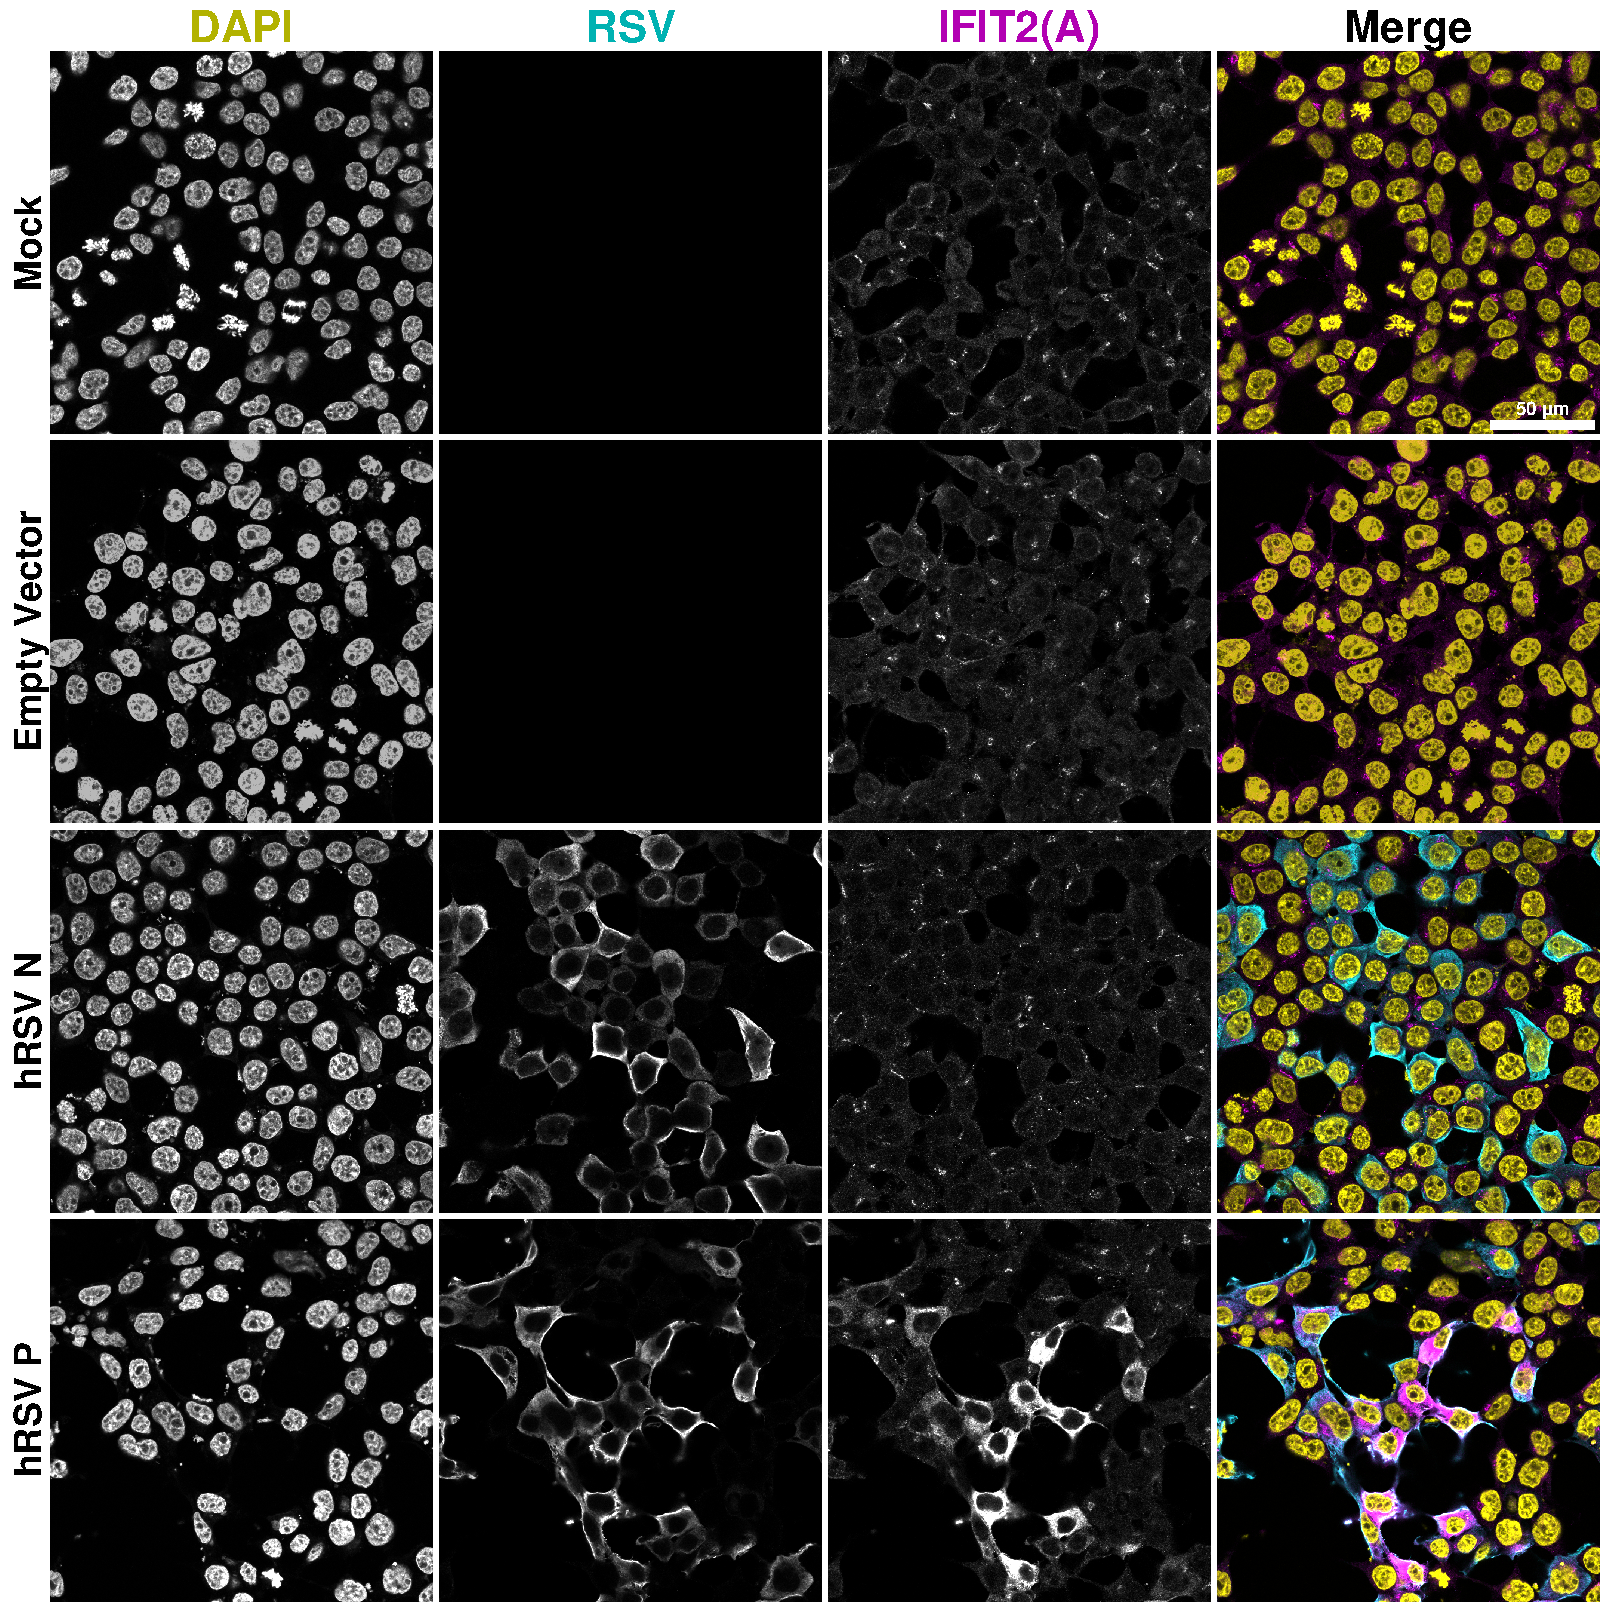
\includegraphics[width=1\linewidth]{09. Chapter 4/Figs/01. pIB/03. IFIT2/01. Single Transfection/01. 293t-ifit2a.pdf}
    \caption[IFIT2(A) Antibody Detects Increased IFIT2 Expression Following hRSV P Transfection.]{\textbf{IFIT2(A) Antibody Detects Increased IFIT2 Expression Following hRSV P Transfection.} HEK293T cells were either mock transfected, or single transfected with empty vector, hRSV N containing plasmid, or hRSV P containing plasmid using TransIT-X2 and were fixed after 24 hours. Cellular nuclei were stained with DAPI (yellow), and cells were double-labelled with either anti-RSV N (cyan), or anti-RSV P (cyan) and anti-IFIT2(A) (magenta) antibodies. The scale bar indicates 50 \(\mu \mbox{m}\).}
    \label{fig:IFIT2(A) Antibody Detects Increased IFIT2 Expression Following hRSV P Transfection}
\end{figure}

\begin{figure}
    \centering
    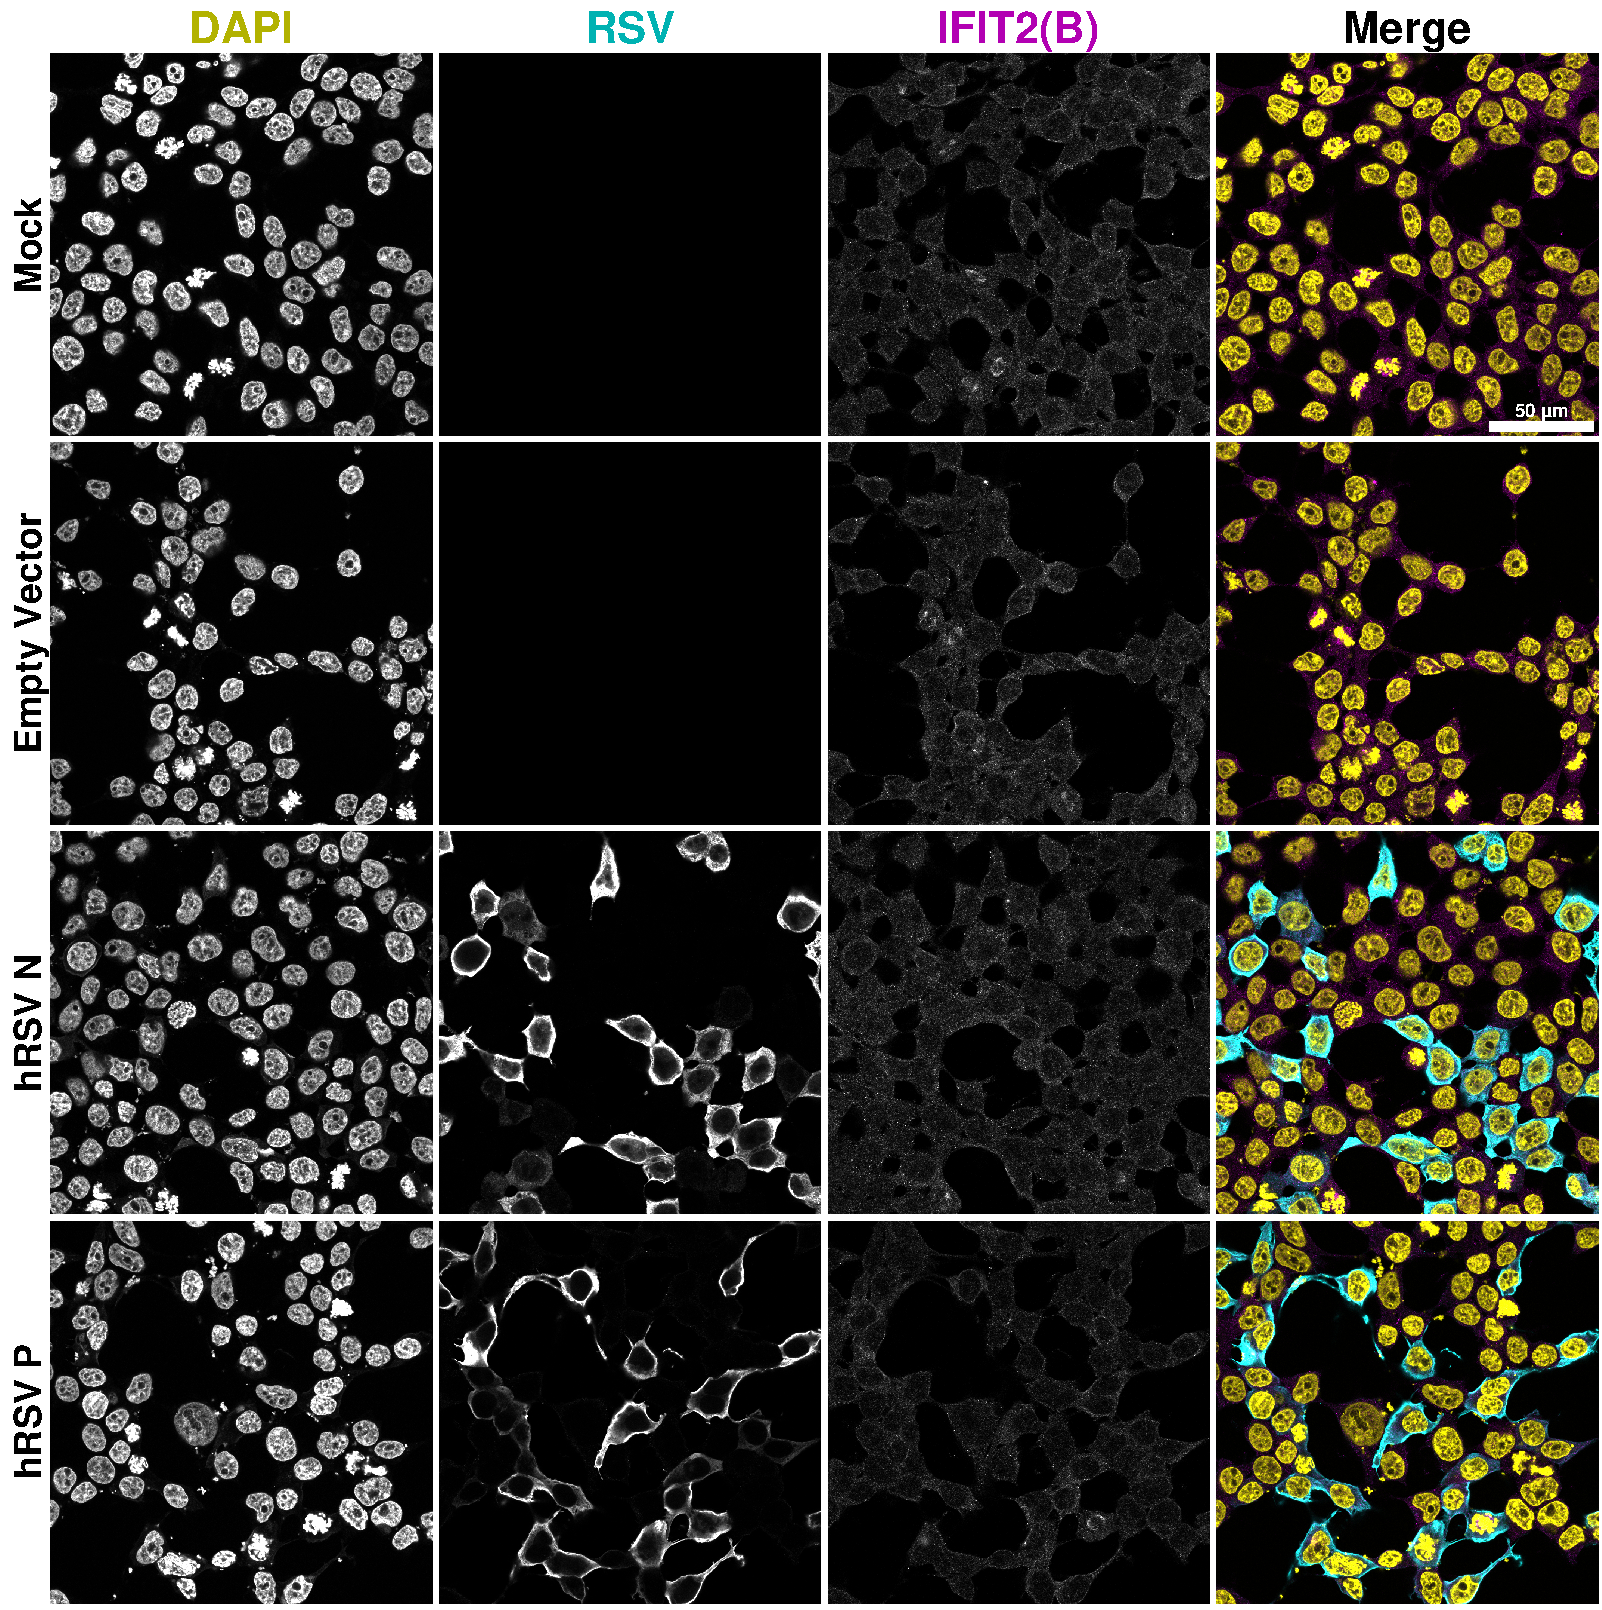
\includegraphics[width=1\linewidth]{09. Chapter 4/Figs/01. pIB/03. IFIT2/01. Single Transfection/02. 293t-ifit2b.pdf}
    \caption[IFIT2(B) Antibody Does Not Detect Increased IFIT2 Expression Following hRSV P Transfection.]{\textbf{IFIT2(B) Antibody Does Not Detect Increased IFIT2 Expression Following hRSV P Transfection.} HEK293T cells were either mock transfected, or single transfected with empty vector, hRSV N containing plasmid, or hRSV P containing plasmid using TransIT-X2 and were fixed after 24 hours. Cellular nuclei were stained with DAPI (yellow), and cells were double-labelled with either anti-RSV N (cyan), or anti-RSV P (cyan) and anti-IFIT2(B) (magenta) antibodies. The scale bar indicates 50 \(\mu \mbox{m}\).}
    \label{fig:IFIT2(B) Antibody Does Not Detect Increased IFIT2 Expression Following hRSV P Transfection}
\end{figure}

While conducting the fundemental control experiments consisting of asssesing the single RSV \textit{N} and \textit{P} transfectons, along with transfections with empty pcDNA3.1 plasmid, while comparing these to mock-transfected cells we have uncovered another differentiation between IFIT2(A) and IFIT2(B) staining. We have observed IFIT2 induction as a response to transfection with hRSV \textit{P}-containing plasmid, which did not occur during the transfection with empty vector or hRSV \textit{N}-containing plasmid. This induction occured only in the cells where we dected hRSV \textit{P} expression. Interesingly, this was only detected using IFIT2(A) (Figure \ref{fig:IFIT2(A) Antibody Detects Increased IFIT2 Expression Following hRSV P Transfection}), while IFIT2(B) staining did not revel this phenotype (Figure \ref{fig:IFIT2(B) Antibody Does Not Detect Increased IFIT2 Expression Following hRSV P Transfection}). We conducted these control experiments for IFIT1, IFIT3, and IFIT5 which revealed staining patter consistent to what IFIT2(B) antibody observed (data not shown). Along to this, we can observe differential subcellular localisation of IFIT2 between the detection of the two antibodies, which is somewhat consistent to what was observed in Chapter \ref{ch:Subcellular Localisation of Endogenous IFIT Proteins in the Context of RSV Inclusion Bodies} in the MDBK cell line. We have observed IFIT2(A)-stained HEK293T mock cells to show perinuclear IFT2 concentrations resembling lipid droplets or aggregosomes, based the definitions and expamples provided by the Human Protien Atlas \cite{Thul2017AProteome}. The IFIT2(B) antibody showed IFIT2 localising to the mitotic spindle. This data poses a few questions. Since the \textit{IFIT} genes should possess similar genomic regulation, through which mechanism does \textit{IFIT2} get induced following RSV \textit{P} exogenous expression? Is this mediated via the direct acxtion of the P protein and thus is this indicative to what happens during infection? This would imply that the \textit{hIFIT2} induction caused by RSV infection (from Chapter \ref{ch:Assessment of Transcriptional Induction of Human IFITs in the Context of RSV}) apperas predominantly in infected, P expressing cells and thus hnts at direct IFIT2 antiviral role against RSV. The other imnportant question is how is it possible that IFIT2(B) antibody is unable to detect this increased nascent IFIT2? If the previously mentioned differential target epitope, based on the IFIT2 interaction partners is correct, this would suggest that IFIT2(B) antibody detects IFIT2 complexes and thus is blind to the newly synthesised IFIT2, which did not have time to for this complexes yet. Further expreiments are required to validate this claim.

\begin{figure}
    \begin{subfigure}{0.495\textwidth}
        \caption{}
        \includegraphics[width=1\linewidth]{09. Chapter 4/Figs/01. pIB/03. IFIT2/02. IFIT2A/01. bar_i2a_293t.pdf}
    \end{subfigure}
    \begin{subfigure}{0.495\textwidth}
        \caption{}
        \includegraphics[width=1\linewidth]{09. Chapter 4/Figs/01. pIB/03. IFIT2/02. IFIT2A/02. box_i2a_293t.pdf}
    \end{subfigure}
    \caption[Observed Phenotypes of Endogenous Human IFIT2 in the Context of hRSV Pseudo Inclusion Bodies in 293T Cell Line, as Detected by IFIT2(A) Antibody.]{\textbf{Observed Phenotypes of Endogenous Human IFIT2 in the Context of hRSV Pseudo Inclusion Bodies in 293T Cell Line, as Detected by IFIT2(A) Antibody.} 293T cells were transfected with hRSV N and P containing plasmids using TransIT-X2 and were fixed after 24 hours. Cells were labelled with anti-RSV N and anti-IFIT2(A) antibodies and imaged on a confocal microscope. Panel (a) shows the percentual proportions of observed phenotypes between hRSV pseudo inclusion bodies and human IFIT2 (81 observations), with the red dotted line denoting the 5\% threshold, marking phenotypes considered relevant above this limit. Panel (b) shows the IB area in \(\mu \mbox{m}^2\) per observed relevant phenotype.}
    \label{fig:Observed Phenotypes of Endogenous Human IFIT2 in the Context of hRSV Pseudo Inclusion Bodies in 293T Cell Line, as Detected by IFIT2(A) Antibody}
\end{figure}

\begin{figure}
    \centering
    \includegraphics[width=1\linewidth]{09. Chapter 4/Figs/01. pIB/03. IFIT2/02. IFIT2A/03. i2a-293t-hnhp.pdf} 
    \caption[Representative Images of Observed Phenotypes of Endogenous Human IFIT2 in the Context of hRSV Pseudo Inclusion Bodies in 293T Cell Line, as Detected by IFIT2(A) Antibody.]{\textbf{Representative Images of Observed Phenotypes of Endogenous Human IFIT2 in the Context of hRSV Pseudo Inclusion Bodies in 293T Cell Line, as Detected by IFIT2(A) Antibody.} 293T cells were transfected with hRSV N and P containing plasmids using TransIT-X2 and were fixed after 24 hours. Cellular nuclei were stained with DAPI (yellow), and cells were double-labelled with anti-RSV N (cyan) and anti-IFIT2(A) (magenta) antibodies. This figure showcases representative examples of relevant phenotypes in the interaction between human IFIT2 and hRSV pseudo-inclusion bodies. These phenotypes are presented in descending order based on their percentage proportions. The scale bar indicates 2 \(\mu \mbox{m}\).}
    \label{fig:Representative Images of Observed Phenotypes of Endogenous Human IFIT2 in the Context of hRSV Pseudo Inclusion Bodies in 293T Cell Line, as Detected by IFIT2(A) Antibody}
\end{figure}

Next, we set to investigate the interaction phenotypes of IFIT2 with RSV pseudo IBs as detected by the two antibodies, firstly focusing on the signal detected by IFIT2(A) antibody. We have obtained 81 observation of human IFIT2 interacting with hRSV pIBs from HEK293T cell line. The observed phenotypes, along with their frequencies of occurances and the pIB sizes associated with phenotypic interactions that occur with higher than 5\% frequency are shown in Figure \ref{fig:Observed Phenotypes of Endogenous Human IFIT2 in the Context of hRSV Pseudo Inclusion Bodies in 293T Cell Line, as Detected by IFIT2(A) Antibody}, with the represpentaitve images of the phenotypes occuring at more than 5\% frequency are shown in Figure \ref{fig:Representative Images of Observed Phenotypes of Endogenous Human IFIT2 in the Context of hRSV Pseudo Inclusion Bodies in 293T Cell Line, as Detected by IFIT2(A) Antibody}. predominantly we have observed IFIT2 to form intra-pIB inclusion, a phenotype that occur in 98\% of cases. In the remaining 2\% of observations we have observed IFIT2 colocalising with the pIB boundry, while being excluded form the pIB centre. The sizes of inclusion-associated pIBs confront to the general distribution of all obsebserved pIBs in HEK293T cell line, ranging from 0.1 \(\mu \mbox{m}^2\) to 25 \(\mu \mbox{m}^2\) in size, with the median area of 2 \(\mu \mbox{m}^2\). Unlike what we observed with monkey IFIT1 and IFIT5, where the inclusion and colocalisation associated with exclusion phenotypes seem to be restricted to small and large pIBs respectively, we do not see this discintion with endogenous human IFIT2. This suggest that IFIT2, as detected by IFIT2(A) antibody seems to form intra-pIB inclusions, irrespective of their size.

\begin{figure}
    \begin{subfigure}{0.495\textwidth}
        \caption{}
        \includegraphics[width=1\linewidth]{09. Chapter 4/Figs/01. pIB/03. IFIT2/02. IFIT2A/04. bar_i2a_vero_hnhp.pdf} 
    \end{subfigure}
    \begin{subfigure}{0.495\textwidth}
        \caption{}
        \includegraphics[width=1\linewidth]{09. Chapter 4/Figs/01. pIB/03. IFIT2/02. IFIT2A/05. box_i2a_vero_hnhp.pdf}
    \end{subfigure}
    \caption[Observed Phenotypes of Endogenous Monkey IFIT2 in the Context of hRSV Pseudo Inclusion Bodies in Vero Cell Line, as Detected by IFIT2(A) Antibody.]{\textbf{Observed Phenotypes of Endogenous Monkey IFIT2 in the Context of hRSV Pseudo Inclusion Bodies in Vero Cell Line, as Detected by IFIT2(A) Antibody.} Vero cells were transfected with hRSV N and P containing plasmids using TransIT-X2 and were fixed after 24 hours. Cells were labelled with anti-RSV N and anti-IFIT2(A) antibodies and imaged on a confocal microscope. Panel (a) shows the percentual proportions of observed phenotypes between hRSV pseudo inclusion bodies and monkey IFIT2 (48 observations), with the red dotted line denoting the 5\% threshold, marking phenotypes considered relevant above this limit. Panel (b) shows the IB area in \(\mu \mbox{m}^2\) per observed relevant phenotype.}
    \label{fig:Observed Phenotypes of Endogenous Monkey IFIT2 in the Context of hRSV Pseudo Inclusion Bodies in Vero Cell Line, as Detected by IFIT2(A) Antibody}
\end{figure}

\begin{figure}
    \centering
    \includegraphics[width=1\linewidth]{09. Chapter 4/Figs/01. pIB/03. IFIT2/02. IFIT2A/06. i2a-vero-hnhp.pdf}  
    \caption[Representative Images of Observed Phenotypes of Endogenous Monkey IFIT2 in the Context of hRSV Pseudo Inclusion Bodies in Vero Cell Line, as Detected by IFIT2(A) Antibody.]{\textbf{Representative Images of Observed Phenotypes of Endogenous Monkey IFIT2 in the Context of hRSV Pseudo Inclusion Bodies in Vero Cell Line, as Detected by IFIT2(A) Antibody.} Vero cells were transfected with hRSV N and P containing plasmids using TransIT-X2 and were fixed after 24 hours. Cellular nuclei were stained with DAPI (yellow), and cells were double-labelled with anti-RSV N (cyan) and anti-IFIT2(A) (magenta) antibodies. This figure showcases representative examples of relevant phenotypes in the interaction between monkey IFIT2 and hRSV pseudo-inclusion bodies. These phenotypes are presented in descending order based on their percentage proportions. The scale bar indicates 2 \(\mu \mbox{m}\).}
    \label{fig:Representative Images of Observed Phenotypes of Endogenous Monkey IFIT2 in the Context of hRSV Pseudo Inclusion Bodies in Vero Cell Line, as Detected by IFIT2(A) Antibody}
\end{figure}

Next we investigated the monkey IFIT2 interaction with hRSV pIBs as detected by the IFIT2(A) antibody. To do this we trnasfected hRSV \textit{N} and \textit{P} containing plasmids to Vero cells. Doing this we have obtained 48 observations, all of which confronted to the inclusion phyenotype (Figure \ref{fig:Observed Phenotypes of Endogenous Monkey IFIT2 in the Context of hRSV Pseudo Inclusion Bodies in Vero Cell Line, as Detected by IFIT2(A) Antibody}, panel a). The measured area of these hRSV pIBs is showin in Figure \ref{fig:Observed Phenotypes of Endogenous Monkey IFIT2 in the Context of hRSV Pseudo Inclusion Bodies in Vero Cell Line, as Detected by IFIT2(A) Antibody}, panel b. The distribution of the pIB sizes is almost indentical to the aggregate dataset of all pIBs observed in Vero cell line, ranging from sub 0.07 \(\mu \mbox{m}^2\) to supra 60 \(\mu \mbox{m}^2\), with the typical value of 1.2 \(\mu \mbox{m}^2\). This data is consistent to what we observed in HEK293T cells. 

\begin{figure}
    \begin{subfigure}{0.495\textwidth}
        \caption{}
        \includegraphics[width=1\linewidth]{09. Chapter 4/Figs/01. pIB/03. IFIT2/02. IFIT2A/07. bar_i2a_vero_bnbp.pdf} 
    \end{subfigure}
    \begin{subfigure}{0.495\textwidth}
        \caption{}
        \includegraphics[width=1\linewidth]{09. Chapter 4/Figs/01. pIB/03. IFIT2/02. IFIT2A/08. box_i2a_vero_bnbp.pdf}
    \end{subfigure}
    \caption[Observed Phenotypes of Endogenous Monkey IFIT2 in the Context of bRSV Pseudo Inclusion Bodies in Vero Cell Line, as Detected by IFIT2(A) Antibody.]{\textbf{Observed Phenotypes of Endogenous Monkey IFIT2 in the Context of bRSV Pseudo Inclusion Bodies in Vero Cell Line, as Detected by IFIT2(A) Antibody.} Vero cells were transfected with bRSV N and P containing plasmids using TransIT-X2 and were fixed after 24 hours. Cells were labelled with anti-RSV N and anti-IFIT2(A) antibodies and imaged on a confocal microscope. Panel (a) shows the percentual proportions of observed phenotypes between bRSV pseudo inclusion bodies and monkey IFIT2 (38 observations), with the red dotted line denoting the 5\% threshold, marking phenotypes considered relevant above this limit. Panel (b) shows the IB area in \(\mu \mbox{m}^2\) per observed relevant phenotype.}
    \label{fig:Observed Phenotypes of Endogenous Monkey IFIT2 in the Context of bRSV Pseudo Inclusion Bodies in Vero Cell Line, as Detected by IFIT2(A) Antibody}
\end{figure}

\begin{figure}
    \centering
    \includegraphics[width=1\linewidth]{09. Chapter 4/Figs/01. pIB/03. IFIT2/02. IFIT2A/09. i2a-vero-bnbp.pdf} 
    \caption[Representative Images of Observed Phenotypes of Endogenous Monkey IFIT2 in the Context of bRSV Pseudo Inclusion Bodies in Vero Cell Line, as Detected by IFIT2(A) Antibody.]{\textbf{Representative Images of Observed Phenotypes of Endogenous Monkey IFIT2 in the Context of bRSV Pseudo Inclusion Bodies in Vero Cell Line, as Detected by IFIT2(A) Antibody.} Vero cells were transfected with bRSV N and P containing plasmids using TransIT-X2 and were fixed after 24 hours. Cellular nuclei were stained with DAPI (yellow), and cells were double-labelled with anti-RSV N (cyan) and anti-IFIT2(A) (magenta) antibodies. This figure showcases representative examples of relevant phenotypes in the interaction between monkey IFIT2 and bRSV pseudo-inclusion bodies. These phenotypes are presented in descending order based on their percentage proportions. The scale bar indicates 2 \(\mu \mbox{m}\).}
    \label{fig:Representative Images of Observed Phenotypes of Endogenous Monkey IFIT2 in the Context of bRSV Pseudo Inclusion Bodies in Vero Cell Line, as Detected by IFIT2(A) Antibody}
\end{figure}

Finally we investigated the monkey IFIT2 interaction with bRSV pIBs as detected by the IFIT2(A) antibody. To do this we trnasfected bRSV \textit{N} and \textit{P} containing plasmids to Vero cells. Doing this we have obtained 38 observations, all of which confronted to the inclusion phyenotype (Figure \ref{fig:Observed Phenotypes of Endogenous Monkey IFIT2 in the Context of bRSV Pseudo Inclusion Bodies in Vero Cell Line, as Detected by IFIT2(A) Antibody}, panel a). The measured area of these bRSV pIBs is showin in Figure \ref{fig:Observed Phenotypes of Endogenous Monkey IFIT2 in the Context of bRSV Pseudo Inclusion Bodies in Vero Cell Line, as Detected by IFIT2(A) Antibody}, panel b. Although the observed pIBs are not a perfect representation of the agglomerate of all pIB observations in the Vero cell line, they span across enough of the pIB size range that we can conclude that monkey IFIT2 forms intra-pIB inclusions regardless of their size. In more detail, their size ranges from 0.12 \(\mu \mbox{m}^2\) to 16 \(\mu \mbox{m}^2\), with the median value of 1.8 \(\mu \mbox{m}^2\). In summary, IFIT2(A) andtibody detects IFIT2 to form intra-pIB inclusion regardles of the host or viral species or the IB size.

\begin{figure}
    \begin{subfigure}{0.495\textwidth}
        \caption{}
        \includegraphics[width=1\linewidth]{09. Chapter 4/Figs/01. pIB/03. IFIT2/03. IFIT2B/01. bar_i2b_293t.pdf} 
    \end{subfigure}
    \begin{subfigure}{0.495\textwidth}
        \caption{}
        \includegraphics[width=1\linewidth]{09. Chapter 4/Figs/01. pIB/03. IFIT2/03. IFIT2B/02. box_i2b_293t.pdf}
    \end{subfigure}
    \caption[Observed Phenotypes of Endogenous Human IFIT2 in the Context of hRSV Pseudo Inclusion Bodies in 293T Cell Line, as Detected by IFIT2(B) Antibody.]{\textbf{Observed Phenotypes of Endogenous Human IFIT2 in the Context of hRSV Pseudo Inclusion Bodies in 293T Cell Line, as Detected by IFIT2(B) Antibody.} 293T cells were transfected with hRSV N and P containing plasmids using TransIT-X2 and were fixed after 24 hours. Cells were labelled with anti-RSV N and anti-IFIT2(B) antibodies and imaged on a confocal microscope. Panel (a) shows the percentual proportions of observed phenotypes between hRSV pseudo inclusion bodies and human IFIT2 (6 observations), with the red dotted line denoting the 5\% threshold, marking phenotypes considered relevant above this limit. Panel (b) shows the IB area in \(\mu \mbox{m}^2\) per observed relevant phenotype.}
    \label{fig:Observed Phenotypes of Endogenous Human IFIT2 in the Context of hRSV Pseudo Inclusion Bodies in 293T Cell Line, as Detected by IFIT2(B) Antibody}
\end{figure}

\begin{figure}
    \centering
    \includegraphics[width=1\linewidth]{09. Chapter 4/Figs/01. pIB/03. IFIT2/03. IFIT2B/03. i2b-293t-hnhp.pdf} 
    \caption[Representative Images of Observed Phenotypes of Endogenous Human IFIT2 in the Context of hRSV Pseudo Inclusion Bodies in 293T Cell Line, as Detected by IFIT2(B) Antibody.]{\textbf{Representative Images of Observed Phenotypes of Endogenous Human IFIT2 in the Context of hRSV Pseudo Inclusion Bodies in 293T Cell Line, as Detected by IFIT2(B) Antibody.} 293T cells were transfected with hRSV N and P containing plasmids using TransIT-X2 and were fixed after 24 hours. Cellular nuclei were stained with DAPI (yellow), and cells were double-labelled with anti-RSV N (cyan) and anti-IFIT2(B) (magenta) antibodies. This figure showcases representative examples of relevant phenotypes in the interaction between human IFIT2 and hRSV pseudo-inclusion bodies. These phenotypes are presented in descending order based on their percentage proportions. The scale bar indicates 2 \(\mu \mbox{m}\).}
    \label{fig:Representative Images of Observed Phenotypes of Endogenous Human IFIT2 in the Context of hRSV Pseudo Inclusion Bodies in 293T Cell Line, as Detected by IFIT2(B) Antibody}
\end{figure}

100
4

\begin{figure}
    \begin{subfigure}{0.495\textwidth}
        \caption{}
        \includegraphics[width=1\linewidth]{09. Chapter 4/Figs/01. pIB/03. IFIT2/03. IFIT2B/04. bar_i2b_vero_hnhp.pdf} 
    \end{subfigure}
    \begin{subfigure}{0.495\textwidth}
        \caption{}
        \includegraphics[width=1\linewidth]{09. Chapter 4/Figs/01. pIB/03. IFIT2/03. IFIT2B/05. box_i2b_vero_hnhp.pdf}
    \end{subfigure}
    \caption[Observed Phenotypes of Endogenous Monkey IFIT2 in the Context of hRSV Pseudo Inclusion Bodies in Vero Cell Line, as Detected by IFIT2(B) Antibody.]{\textbf{Observed Phenotypes of Endogenous Monkey IFIT2 in the Context of hRSV Pseudo Inclusion Bodies in Vero Cell Line, as Detected by IFIT2(B) Antibody.} Vero cells were transfected with hRSV N and P containing plasmids using TransIT-X2 and were fixed after 24 hours. Cells were labelled with anti-RSV N and anti-IFIT2(B) antibodies and imaged on a confocal microscope. Panel (a) shows the percentual proportions of observed phenotypes between hRSV pseudo inclusion bodies and monkey IFIT2 (76 observations), with the red dotted line denoting the 5\% threshold, marking phenotypes considered relevant above this limit. Panel (b) shows the IB area in \(\mu \mbox{m}^2\) per observed relevant phenotype.}
    \label{fig:Observed Phenotypes of Endogenous Monkey IFIT2 in the Context of hRSV Pseudo Inclusion Bodies in Vero Cell Line, as Detected by IFIT2(B) Antibody}
\end{figure}

\begin{figure}
    \centering
    \includegraphics[width=1\linewidth]{09. Chapter 4/Figs/01. pIB/03. IFIT2/03. IFIT2B/06. i2b-vero-hnhp.pdf} 
    \caption[Representative Images of Observed Phenotypes of Endogenous Monkey IFIT2 in the Context of hRSV Pseudo Inclusion Bodies in Vero Cell Line, as Detected by IFIT2(B) Antibody.]{\textbf{Representative Images of Observed Phenotypes of Endogenous Monkey IFIT2 in the Context of hRSV Pseudo Inclusion Bodies in Vero Cell Line, as Detected by IFIT2(B) Antibody.} Vero cells were transfected with hRSV N and P containing plasmids using TransIT-X2 and were fixed after 24 hours. Cellular nuclei were stained with DAPI (yellow), and cells were double-labelled with anti-RSV N (cyan) and anti-IFIT2(B) (magenta) antibodies. This figure showcases representative examples of relevant phenotypes in the interaction between monkey IFIT2 and hRSV pseudo-inclusion bodies. These phenotypes are presented in descending order based on their percentage proportions. The scale bar indicates 2 \(\mu \mbox{m}\).}
    \label{fig:Representative Images of Observed Phenotypes of Endogenous Monkey IFIT2 in the Context of hRSV Pseudo Inclusion Bodies in Vero Cell Line, as Detected by IFIT2(B) Antibody}
\end{figure}

91 9
2 0.63


% summary
Both endogenous human and monkey IFIT2 forms inclusions inside human RSV pseudo-IBs. Monkey IFIT2 also colocalises to the pIB filamentous network (this structure was not observed in the human experiment). The identical staining can be observed in monkey cells with overexpressed human IFIT2-FLAG.

Endogenous monkey IFIT2 is excluded from human pIB and the pIB associated filamentous network. Overexpressed human IFIT2-FLAG is detected by the antibody and shows inclusions inside the human pIB structures, which is consistent to data from IFIT2(A) staining and FLAG staining of IFIT2-FLAG overexpressed samples. Interestingly, IFIT2(B) antibody shows exclusion from the pIB filamentous network, which was colocalised by IFIT2(A) and FLAG antibodies.

% exogenous
Monkey cells transfected with human RSV N and P, along with human IFIT2-FLAG show concentration within the pIB structures as well as the pIB filamentous network. In this experiment we are detecting both human and monkey IFIT2, however we can see a huge difference in IFIT2 expression between some cells (bottom panel; cells in the periphery of the picture), suggesting that what we are mainly detecting is the overexpressed human IFIT2-FLAG.

\begin{figure}
    \begin{subfigure}{0.495\textwidth}
        \caption{}
        \includegraphics[width=1\linewidth]{09. Chapter 4/Figs/01. pIB/03. IFIT2/04. IFIT2-FLAG/01. IFIT2A/01. bar_i2a_hnhp.pdf} 
    \end{subfigure}
    \begin{subfigure}{0.495\textwidth}
        \caption{}
        \includegraphics[width=1\linewidth]{09. Chapter 4/Figs/01. pIB/03. IFIT2/04. IFIT2-FLAG/01. IFIT2A/02. box_i2a_hnhp.pdf}
    \end{subfigure}
    \caption[Observed Phenotypes of Exogenous Human IFIT2 in the Context of hRSV Pseudo Inclusion Bodies in Vero Cell Line, as Detected by IFIT2(A) Antibody.]{\textbf{Observed Phenotypes of Exogenous Human IFIT2 in the Context of hRSV Pseudo Inclusion Bodies in Vero Cell Line, as Detected by IFIT2(A) Antibody.} Vero cells were transfected with hRSV N and P, along with human IFIT2-FLAG containing plasmids using TransIT-X2 and were fixed after 24 hours. Cells were labelled with anti-RSV N and anti-IFIT2(A) antibodies and imaged on a confocal microscope. Panel (a) shows the percentual proportions of observed phenotypes between hRSV pseudo inclusion bodies and exogenous human IFIT2 (56 observations), with the red dotted line denoting the 5\% threshold, marking phenotypes considered relevant above this limit. Panel (b) shows the IB area in \(\mu \mbox{m}^2\) per observed relevant phenotype.}
    \label{fig:Observed Phenotypes of Exogenous Human IFIT2 in the Context of hRSV Pseudo Inclusion Bodies in Vero Cell Line, as Detected by IFIT2(A) Antibody}
\end{figure}

\begin{figure}
    \centering
    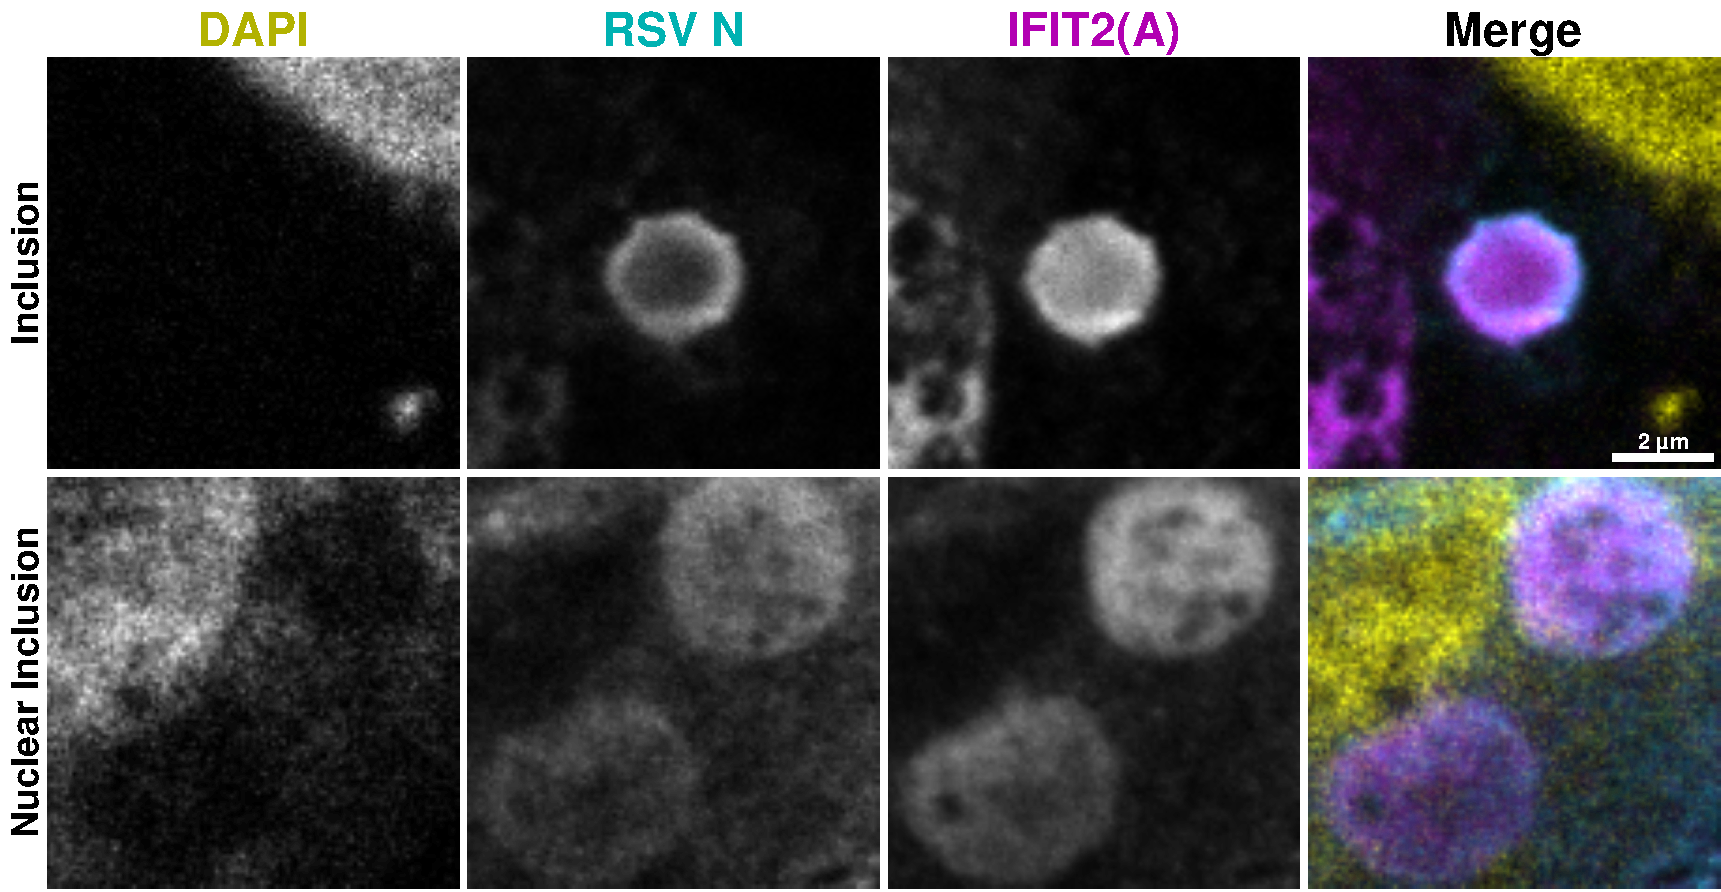
\includegraphics[width=1\linewidth]{09. Chapter 4/Figs/01. pIB/03. IFIT2/04. IFIT2-FLAG/01. IFIT2A/03. i2a-hi2f-hnhp.pdf}
    \caption[Representative Images of Observed Phenotypes of Exogenous Human IFIT2 in the Context of hRSV Pseudo Inclusion Bodies in Vero Cell Line, as Detected by IFIT2(A) Antibody.]{\textbf{Representative Images of Observed Phenotypes of Exogenous Human IFIT2 in the Context of hRSV Pseudo Inclusion Bodies in Vero Cell Line, as Detected by IFIT2(A) Antibody.} Vero cells were transfected with hRSV N and P, along with human IFIT2-FLAG containing plasmids using TransIT-X2 and were fixed after 24 hours. Cellular nuclei were stained with DAPI (yellow), and cells were double-labelled with anti-RSV N (cyan) and anti-IFIT2(A) (magenta) antibodies. This figure showcases representative examples of relevant phenotypes in the interaction between exogenous human IFIT2 and hRSV pseudo-inclusion bodies. These phenotypes are presented in descending order based on their percentage proportions. The scale bar indicates 2 \(\mu \mbox{m}\).}
    \label{fig:Representative Images of Observed Phenotypes of Exogenous Human IFIT2 in the Context of hRSV Pseudo Inclusion Bodies in Vero Cell Line, as Detected by IFIT2(A) Antibody}
\end{figure}

100
0.9

Monkey cells transfected with human RSV N and P, along with human IFIT2-FLAG show concentration within the pIB structures but show exclusion from the pIB filamentous network (or partial colocalsiation?). This suggest that the IFIT2(B) antibody can indeed detect IFIT2 but the overexpressed IFIT2 observed between the inclusion and the one interacting with the filamentous network is somehow different (epitope masking?).

\begin{figure}
    \begin{subfigure}{0.495\textwidth}
        \caption{}
        \includegraphics[width=1\linewidth]{09. Chapter 4/Figs/01. pIB/03. IFIT2/04. IFIT2-FLAG/02. IFIT2B/01. bar_i2b_hnhp.pdf}
    \end{subfigure}
    \begin{subfigure}{0.495\textwidth}
        \caption{}
        \includegraphics[width=1\linewidth]{09. Chapter 4/Figs/01. pIB/03. IFIT2/04. IFIT2-FLAG/02. IFIT2B/02. box_i2a_hnhp.pdf}
    \end{subfigure}
    \caption[Observed Phenotypes of Exogenous Human IFIT2 in the Context of hRSV Pseudo Inclusion Bodies in Vero Cell Line, as Detected by IFIT2(B) Antibody.]{\textbf{Observed Phenotypes of Exogenous Human IFIT2 in the Context of hRSV Pseudo Inclusion Bodies in Vero Cell Line, as Detected by IFIT2(B) Antibody.} Vero cells were transfected with hRSV N and P, along with human IFIT2-FLAG containing plasmids using TransIT-X2 and were fixed after 24 hours. Cells were labelled with anti-RSV N and anti-IFIT2(B) antibodies and imaged on a confocal microscope. Panel (a) shows the percentual proportions of observed phenotypes between hRSV pseudo inclusion bodies and exogenous human IFIT2 (44 observations), with the red dotted line denoting the 5\% threshold, marking phenotypes considered relevant above this limit. Panel (b) shows the IB area in \(\mu \mbox{m}^2\) per observed relevant phenotype.}
    \label{fig:Observed Phenotypes of Exogenous Human IFIT2 in the Context of hRSV Pseudo Inclusion Bodies in Vero Cell Line, as Detected by IFIT2(B) Antibody}
\end{figure}

\begin{figure}
    \centering
    \includegraphics[width=1\linewidth]{09. Chapter 4/Figs/01. pIB/03. IFIT2/04. IFIT2-FLAG/02. IFIT2B/03. i2b-hi2f-hnhp.pdf}
    \caption[Representative Images of Observed Phenotypes of Exogenous Human IFIT2 in the Context of hRSV Pseudo Inclusion Bodies in Vero Cell Line, as Detected by IFIT2(B) Antibody.]{\textbf{Representative Images of Observed Phenotypes of Exogenous Human IFIT2 in the Context of hRSV Pseudo Inclusion Bodies in Vero Cell Line, as Detected by IFIT2(B) Antibody.} Vero cells were transfected with hRSV N and P, along with human IFIT2-FLAG containing plasmids using TransIT-X2 and were fixed after 24 hours. Cellular nuclei were stained with DAPI (yellow), and cells were double-labelled with anti-RSV N (cyan) and anti-IFIT2(B) (magenta) antibodies. This figure showcases representative examples of relevant phenotypes in the interaction between exogenous human IFIT2 and hRSV pseudo-inclusion bodies. These phenotypes are presented in descending order based on their percentage proportions. The scale bar indicates 2 \(\mu \mbox{m}\).}
    \label{fig:Representative Images of Observed Phenotypes of Exogenous Human IFIT2 in the Context of hRSV Pseudo Inclusion Bodies in Vero Cell Line, as Detected by IFIT2(B) Antibody}
\end{figure}

50 47
3.2 0.4

Exogenously expressed human IFIT2 colocalises with the pIB associated filamentous net (top panel). It also forms inclusion inside the human pIB structures. This data is consistent with what we observed with IFIT2(A) antibody. IFIT2 also seems to occasionally form aggregates/spots (highlighted by arrows). These could be functional or just aggregates caused by overexpression, we do not know.

\begin{figure}
    \begin{subfigure}{0.495\textwidth}
        \caption{}
        \includegraphics[width=1\linewidth]{09. Chapter 4/Figs/01. pIB/03. IFIT2/04. IFIT2-FLAG/03. FLAG/01. bar_hi2f_hnhp.pdf}
    \end{subfigure}
    \begin{subfigure}{0.495\textwidth}
        \caption{}
        \includegraphics[width=1\linewidth]{09. Chapter 4/Figs/01. pIB/03. IFIT2/04. IFIT2-FLAG/03. FLAG/02. box_hi2f_hnhp.pdf}
    \end{subfigure}
    \caption[Observed Phenotypes of Exogenous Human IFIT2 in the Context of hRSV Pseudo Inclusion Bodies in Vero Cell Line, as Detected by FLAG Antibody.]{\textbf{Observed Phenotypes of Exogenous Human IFIT2 in the Context of hRSV Pseudo Inclusion Bodies in Vero Cell Line, as Detected by FLAG Antibody.} Vero cells were transfected with hRSV N and P, along with human IFIT2-FLAG containing plasmids using TransIT-X2 and were fixed after 24 hours. Cells were labelled with anti-RSV N and anti-FLAG antibodies and imaged on a confocal microscope. Panel (a) shows the percentual proportions of observed phenotypes between hRSV pseudo inclusion bodies and exogenous human IFIT2 (116 observations), with the red dotted line denoting the 5\% threshold, marking phenotypes considered relevant above this limit. Panel (b) shows the IB area in \(\mu \mbox{m}^2\) per observed relevant phenotype.}
    \label{fig:Observed Phenotypes of Exogenous Human IFIT2 in the Context of hRSV Pseudo Inclusion Bodies in Vero Cell Line, as Detected by FLAG Antibody}
\end{figure}

\begin{figure}
    \centering
    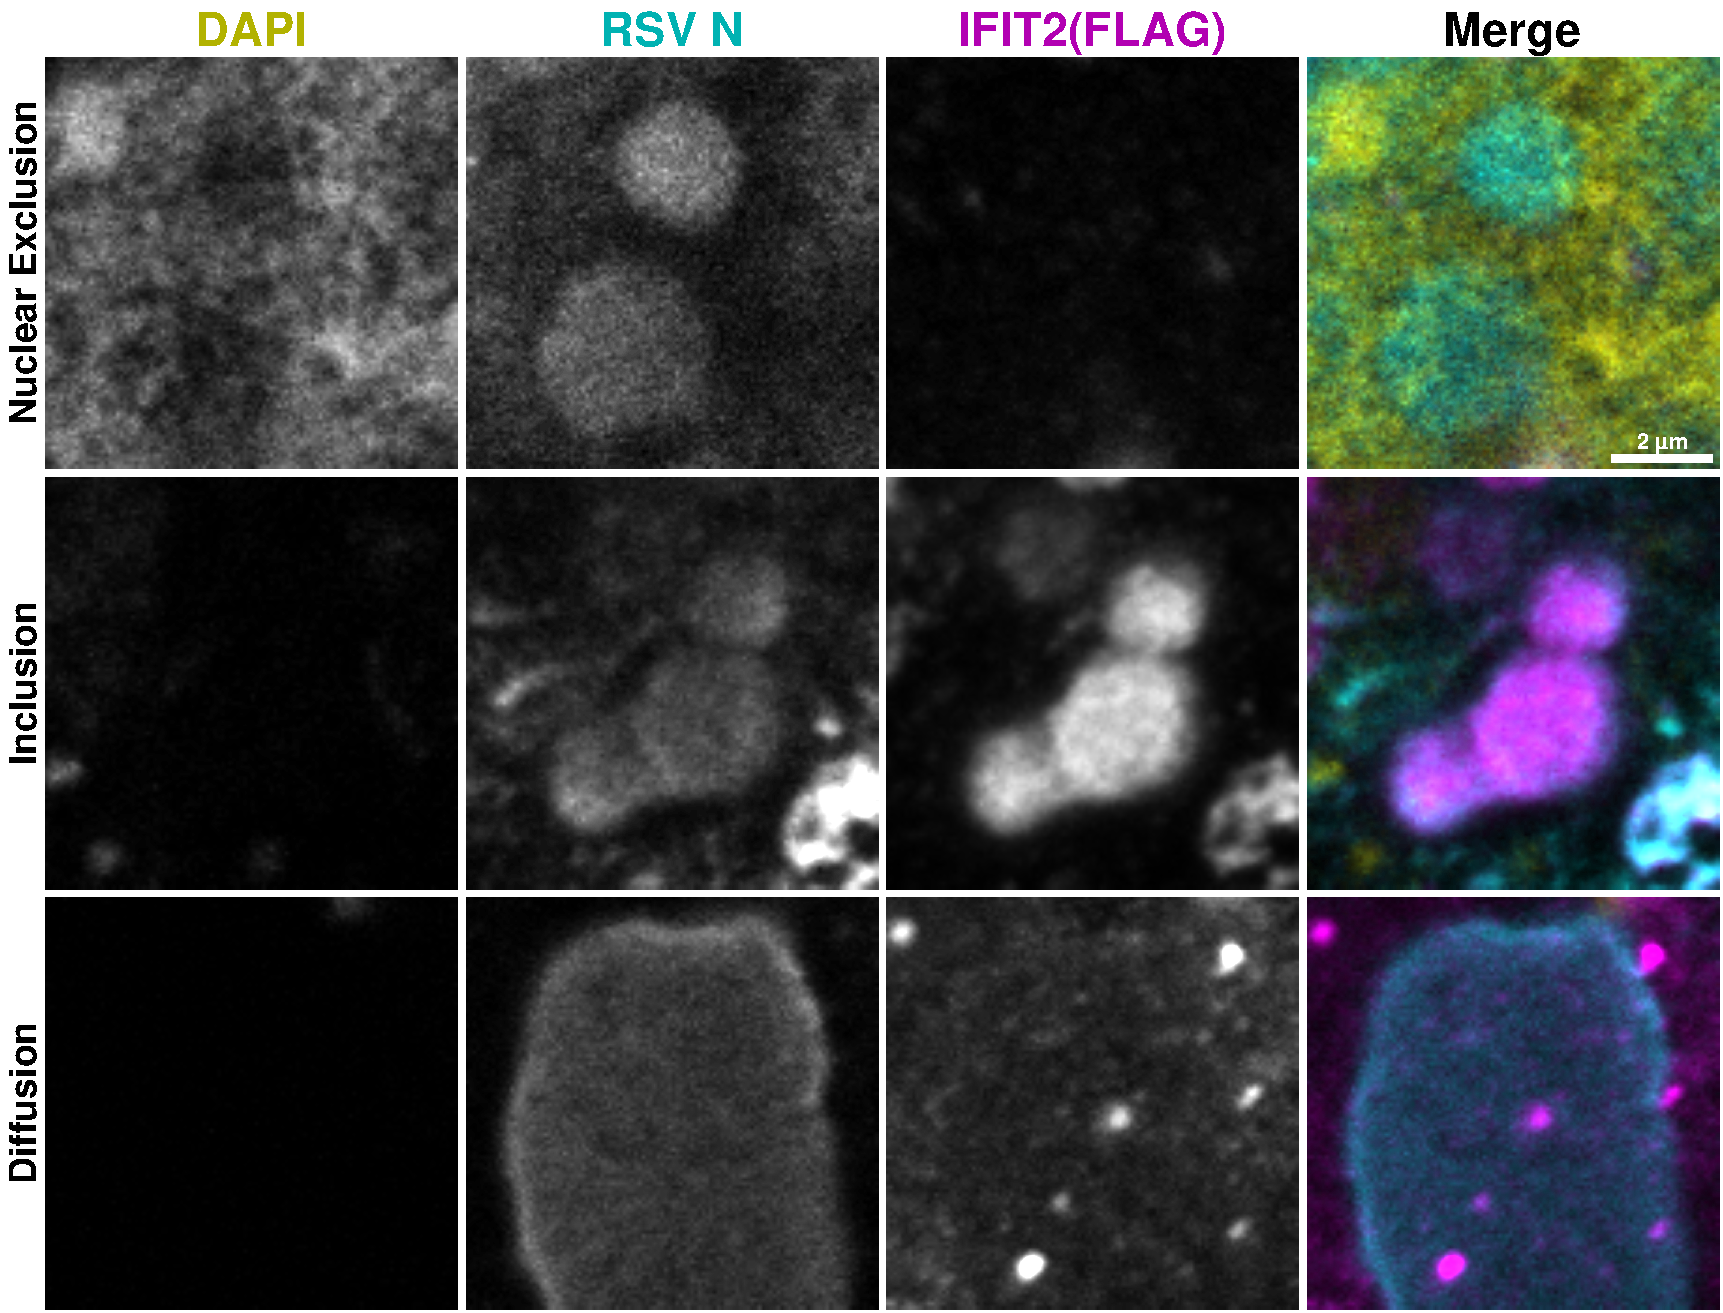
\includegraphics[width=1\linewidth]{09. Chapter 4/Figs/01. pIB/03. IFIT2/04. IFIT2-FLAG/03. FLAG/03. hi2f-hnhp.pdf}
    \caption[Representative Images of Observed Phenotypes of Exogenous Human IFIT2 in the Context of hRSV Pseudo Inclusion Bodies in Vero Cell Line, as Detected by FLAG Antibody.]{\textbf{Representative Images of Observed Phenotypes of Exogenous Human IFIT2 in the Context of hRSV Pseudo Inclusion Bodies in Vero Cell Line, as Detected by FLAG Antibody.} Vero cells were transfected with hRSV N and P, along with human IFIT2-FLAG containing plasmids using TransIT-X2 and were fixed after 24 hours. Cellular nuclei were stained with DAPI (yellow), and cells were double-labelled with anti-RSV N (cyan) and anti-FLAG (magenta) antibodies. This figure showcases representative examples of relevant phenotypes in the interaction between exogenous human IFIT2 and hRSV pseudo-inclusion bodies. These phenotypes are presented in descending order based on their percentage proportions. The scale bar indicates 2 \(\mu \mbox{m}\).}
    \label{fig:Representative Images of Observed Phenotypes of Exogenous Human IFIT2 in the Context of hRSV Pseudo Inclusion Bodies in Vero Cell Line, as Detected by FLAG Antibody}
\end{figure}

49 35 21
0.23 2.1 0.7

Exogenous bovine IFIT2 colocalises with the edge of human pIB structures. This is unusual as human IFIT2 data suggest inclusions with regards to pIBs.  

\begin{figure}
    \begin{subfigure}{0.495\textwidth}
        \caption{}
        \includegraphics[width=1\linewidth]{09. Chapter 4/Figs/01. pIB/03. IFIT2/04. IFIT2-FLAG/03. FLAG/04. bar_bi2f_hnhp.pdf} 
    \end{subfigure}
    \begin{subfigure}{0.495\textwidth}
        \caption{}
        \includegraphics[width=1\linewidth]{09. Chapter 4/Figs/01. pIB/03. IFIT2/04. IFIT2-FLAG/03. FLAG/05. box_bi2f_hnhp.pdf}
    \end{subfigure}
    \caption[Observed Phenotypes of Exogenous Bovine IFIT2 in the Context of hRSV Pseudo Inclusion Bodies in Vero Cell Line, as Detected by FLAG Antibody.]{\textbf{Observed Phenotypes of Exogenous Bovine IFIT2 in the Context of hRSV Pseudo Inclusion Bodies in Vero Cell Line, as Detected by FLAG Antibody.} Vero cells were transfected with hRSV N and P, along with bovine IFIT2-FLAG containing plasmids using TransIT-X2 and were fixed after 24 hours. Cells were labelled with anti-RSV N and anti-FLAG antibodies and imaged on a confocal microscope. Panel (a) shows the percentual proportions of observed phenotypes between hRSV pseudo inclusion bodies and exogenous bovine IFIT2 (142 observations), with the red dotted line denoting the 5\% threshold, marking phenotypes considered relevant above this limit. Panel (b) shows the IB area in \(\mu \mbox{m}^2\) per observed relevant phenotype.}
    \label{fig:Observed Phenotypes of Exogenous Bovine IFIT2 in the Context of hRSV Pseudo Inclusion Bodies in Vero Cell Line, as Detected by FLAG Antibody}
\end{figure}

\begin{figure}
    \centering
    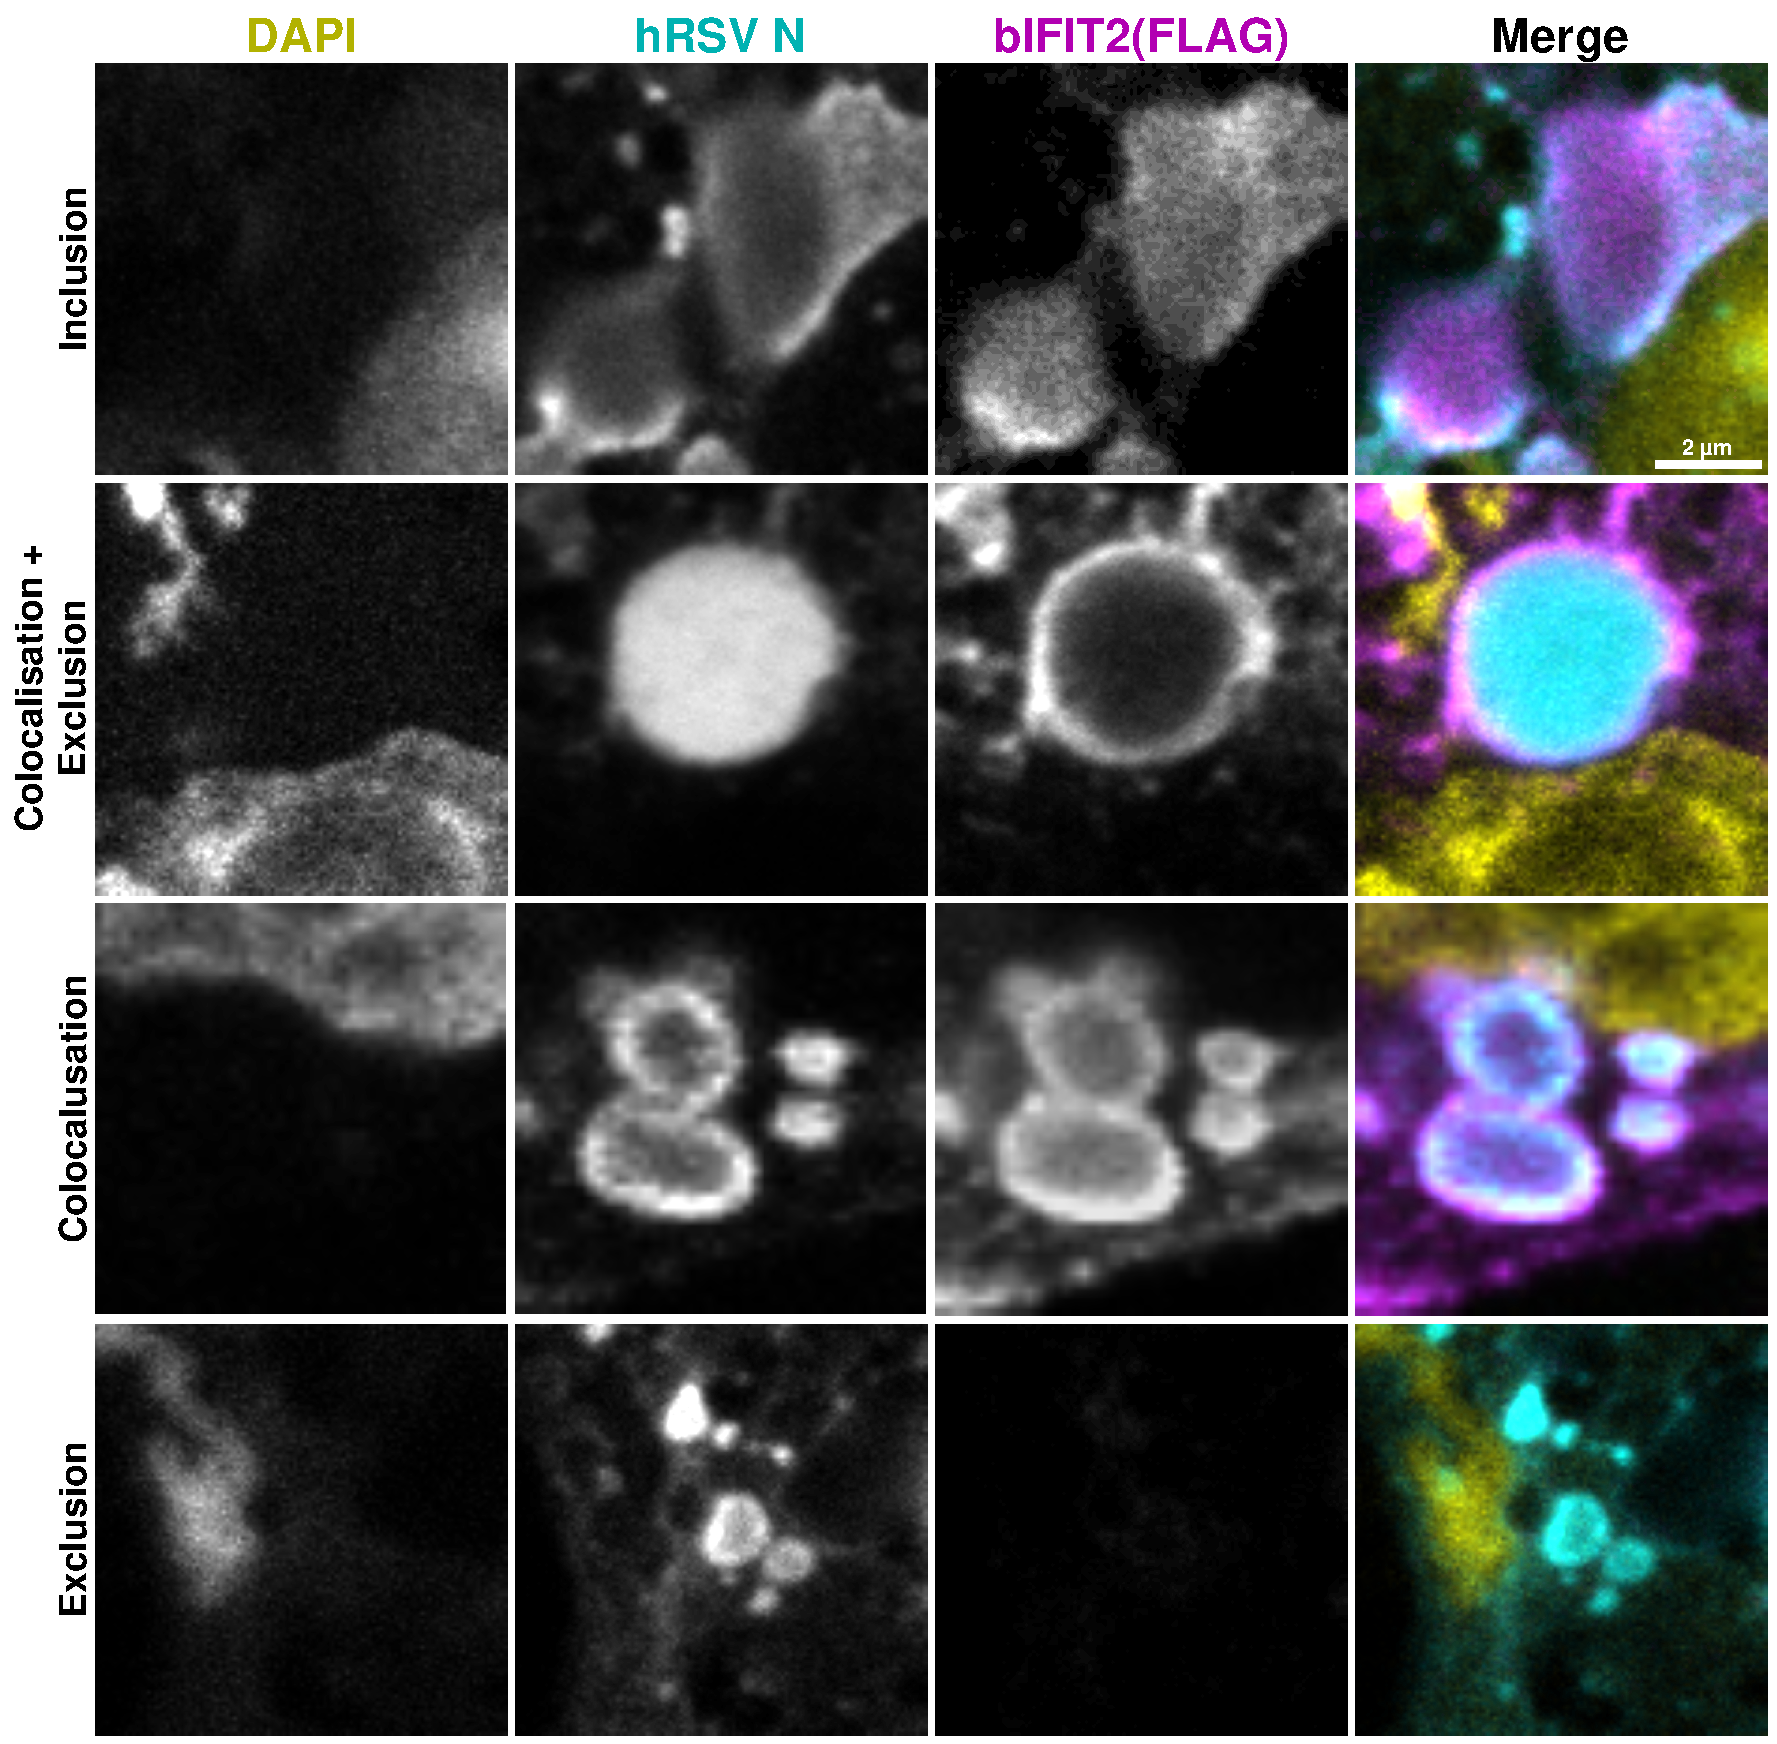
\includegraphics[width=1\linewidth]{09. Chapter 4/Figs/01. pIB/03. IFIT2/04. IFIT2-FLAG/03. FLAG/06. bi2f-hnhp.pdf}
    \caption[Representative Images of Observed Phenotypes of Exogenous Bovine IFIT2 in the Context of hRSV Pseudo Inclusion Bodies in Vero Cell Line, as Detected by FLAG Antibody.]{\textbf{Representative Images of Observed Phenotypes of Exogenous Bovine IFIT2 in the Context of hRSV Pseudo Inclusion Bodies in Vero Cell Line, as Detected by FLAG Antibody.} Vero cells were transfected with hRSV N and P, along with bovine IFIT2-FLAG containing plasmids using TransIT-X2 and were fixed after 24 hours. Cellular nuclei were stained with DAPI (yellow), and cells were double-labelled with anti-RSV N (cyan) and anti-FLAG (magenta) antibodies. This figure showcases representative examples of relevant phenotypes in the interaction between exogenous bovine IFIT2 and hRSV pseudo-inclusion bodies. These phenotypes are presented in descending order based on their percentage proportions. The scale bar indicates 2 \(\mu \mbox{m}\).}
    \label{fig:Representative Images of Observed Phenotypes of Exogenous Bovine IFIT2 in the Context of hRSV Pseudo Inclusion Bodies in Vero Cell Line, as Detected by FLAG Antibody}
\end{figure}

46 31 12 6
1 2.8 2.8 1.7

\begin{figure}
    \begin{subfigure}{0.495\textwidth}
        \caption{}
        \includegraphics[width=1\linewidth]{09. Chapter 4/Figs/01. pIB/03. IFIT2/04. IFIT2-FLAG/03. FLAG/07. bar_bi2f_bnbp.pdf} 
    \end{subfigure}
    \begin{subfigure}{0.495\textwidth}
        \caption{}
        \includegraphics[width=1\linewidth]{09. Chapter 4/Figs/01. pIB/03. IFIT2/04. IFIT2-FLAG/03. FLAG/08. box_bi2f_bnbp.pdf}
    \end{subfigure}
    \caption[Observed Phenotypes of Exogenous Bovine IFIT2 in the Context of bRSV Pseudo Inclusion Bodies in Vero Cell Line, as Detected by FLAG Antibody.]{\textbf{Observed Phenotypes of Exogenous Bovine IFIT2 in the Context of bRSV Pseudo Inclusion Bodies in Vero Cell Line, as Detected by FLAG Antibody.} Vero cells were transfected with bRSV N and P, along with bovine IFIT2-FLAG containing plasmids using TransIT-X2 and were fixed after 24 hours. Cells were labelled with anti-RSV N and anti-FLAG antibodies and imaged on a confocal microscope. Panel (a) shows the percentual proportions of observed phenotypes between bRSV pseudo inclusion bodies and exogenous bovine IFIT2 (22 observations), with the red dotted line denoting the 5\% threshold, marking phenotypes considered relevant above this limit. Panel (b) shows the IB area in \(\mu \mbox{m}^2\) per observed relevant phenotype.}
    \label{fig:Observed Phenotypes of Exogenous Bovine IFIT2 in the Context of bRSV Pseudo Inclusion Bodies in Vero Cell Line, as Detected by FLAG Antibody}
\end{figure}

\begin{figure}
    \centering
    \includegraphics[width=1\linewidth]{09. Chapter 4/Figs/01. pIB/03. IFIT2/04. IFIT2-FLAG/03. FLAG/09. bi2f-bnbp.pdf}
    \caption[Representative Images of Observed Phenotypes of Exogenous Bovine IFIT2 in the Context of bRSV Pseudo Inclusion Bodies in Vero Cell Line, as Detected by FLAG Antibody.]{\textbf{Representative Images of Observed Phenotypes of Exogenous Bovine IFIT2 in the Context of bRSV Pseudo Inclusion Bodies in Vero Cell Line, as Detected by FLAG Antibody.} Vero cells were transfected with bRSV N and P, along with bovine IFIT2-FLAG containing plasmids using TransIT-X2 and were fixed after 24 hours. Cellular nuclei were stained with DAPI (yellow), and cells were double-labelled with anti-RSV N (cyan) and anti-FLAG (magenta) antibodies. This figure showcases representative examples of relevant phenotypes in the interaction between exogenous bovine IFIT2 and bRSV pseudo-inclusion bodies. These phenotypes are presented in descending order based on their percentage proportions. The scale bar indicates 2 \(\mu \mbox{m}\).}
    \label{fig:Representative Images of Observed Phenotypes of Exogenous Bovine IFIT2 in the Context of bRSV Pseudo Inclusion Bodies in Vero Cell Line, as Detected by FLAG Antibody}
\end{figure}

100
0.41

what we tried that did not work - pib with hi2f and i3-ha (ha signal not strong enough or trasnfection didnt work)


what did not work - hif2 and bovine pIB

%infection

\begin{figure}
    \begin{subfigure}{0.495\textwidth}
        \caption{}
        \includegraphics[width=1\linewidth]{09. Chapter 4/Figs/02. Overexpression/02. IFIT2/01. bar_hi2f_hrsv.pdf} 
    \end{subfigure}
    \begin{subfigure}{0.495\textwidth}
        \caption{}
        \includegraphics[width=1\linewidth]{09. Chapter 4/Figs/02. Overexpression/02. IFIT2/02. box_hi2f_hrsv.pdf}
    \end{subfigure}
    \caption[Observed Phenotypes of Exogenous hIFIT2 in the Context of hRSV Inclusion Bodies in Vero Cell Line.]{\textbf{Observed Phenotypes of Exogenous hIFIT2 in the Context of hRSV Inclusion Bodies in Vero Cell Line.} Vero cells were infected with human RSV at MOI 1. 24 HPI, the cells were transfected with hIFIT2-FLAG containing plasmids using TransIT-X2 and were fixed after a further 24 hours. Cells were labelled with anti-RSV N and anti-FLAG antibodies and imaged on a confocal microscope. Panel (a) shows the percentual proportions of observed phenotypes between hRSV inclusion bodies and exogenous hIFIT2 (155 observations), with the red dotted line denoting the 5\% threshold, marking phenotypes considered relevant above this limit. Panel (b) shows the IB area in \(\mu \mbox{m}^2\) per observed relevant phenotype.}
    \label{fig:Observed Phenotypes of Exogenous hIFIT2 in the Context of hRSV Inclusion Bodies in Vero Cell Line}
\end{figure}

\begin{figure}
    \centering
    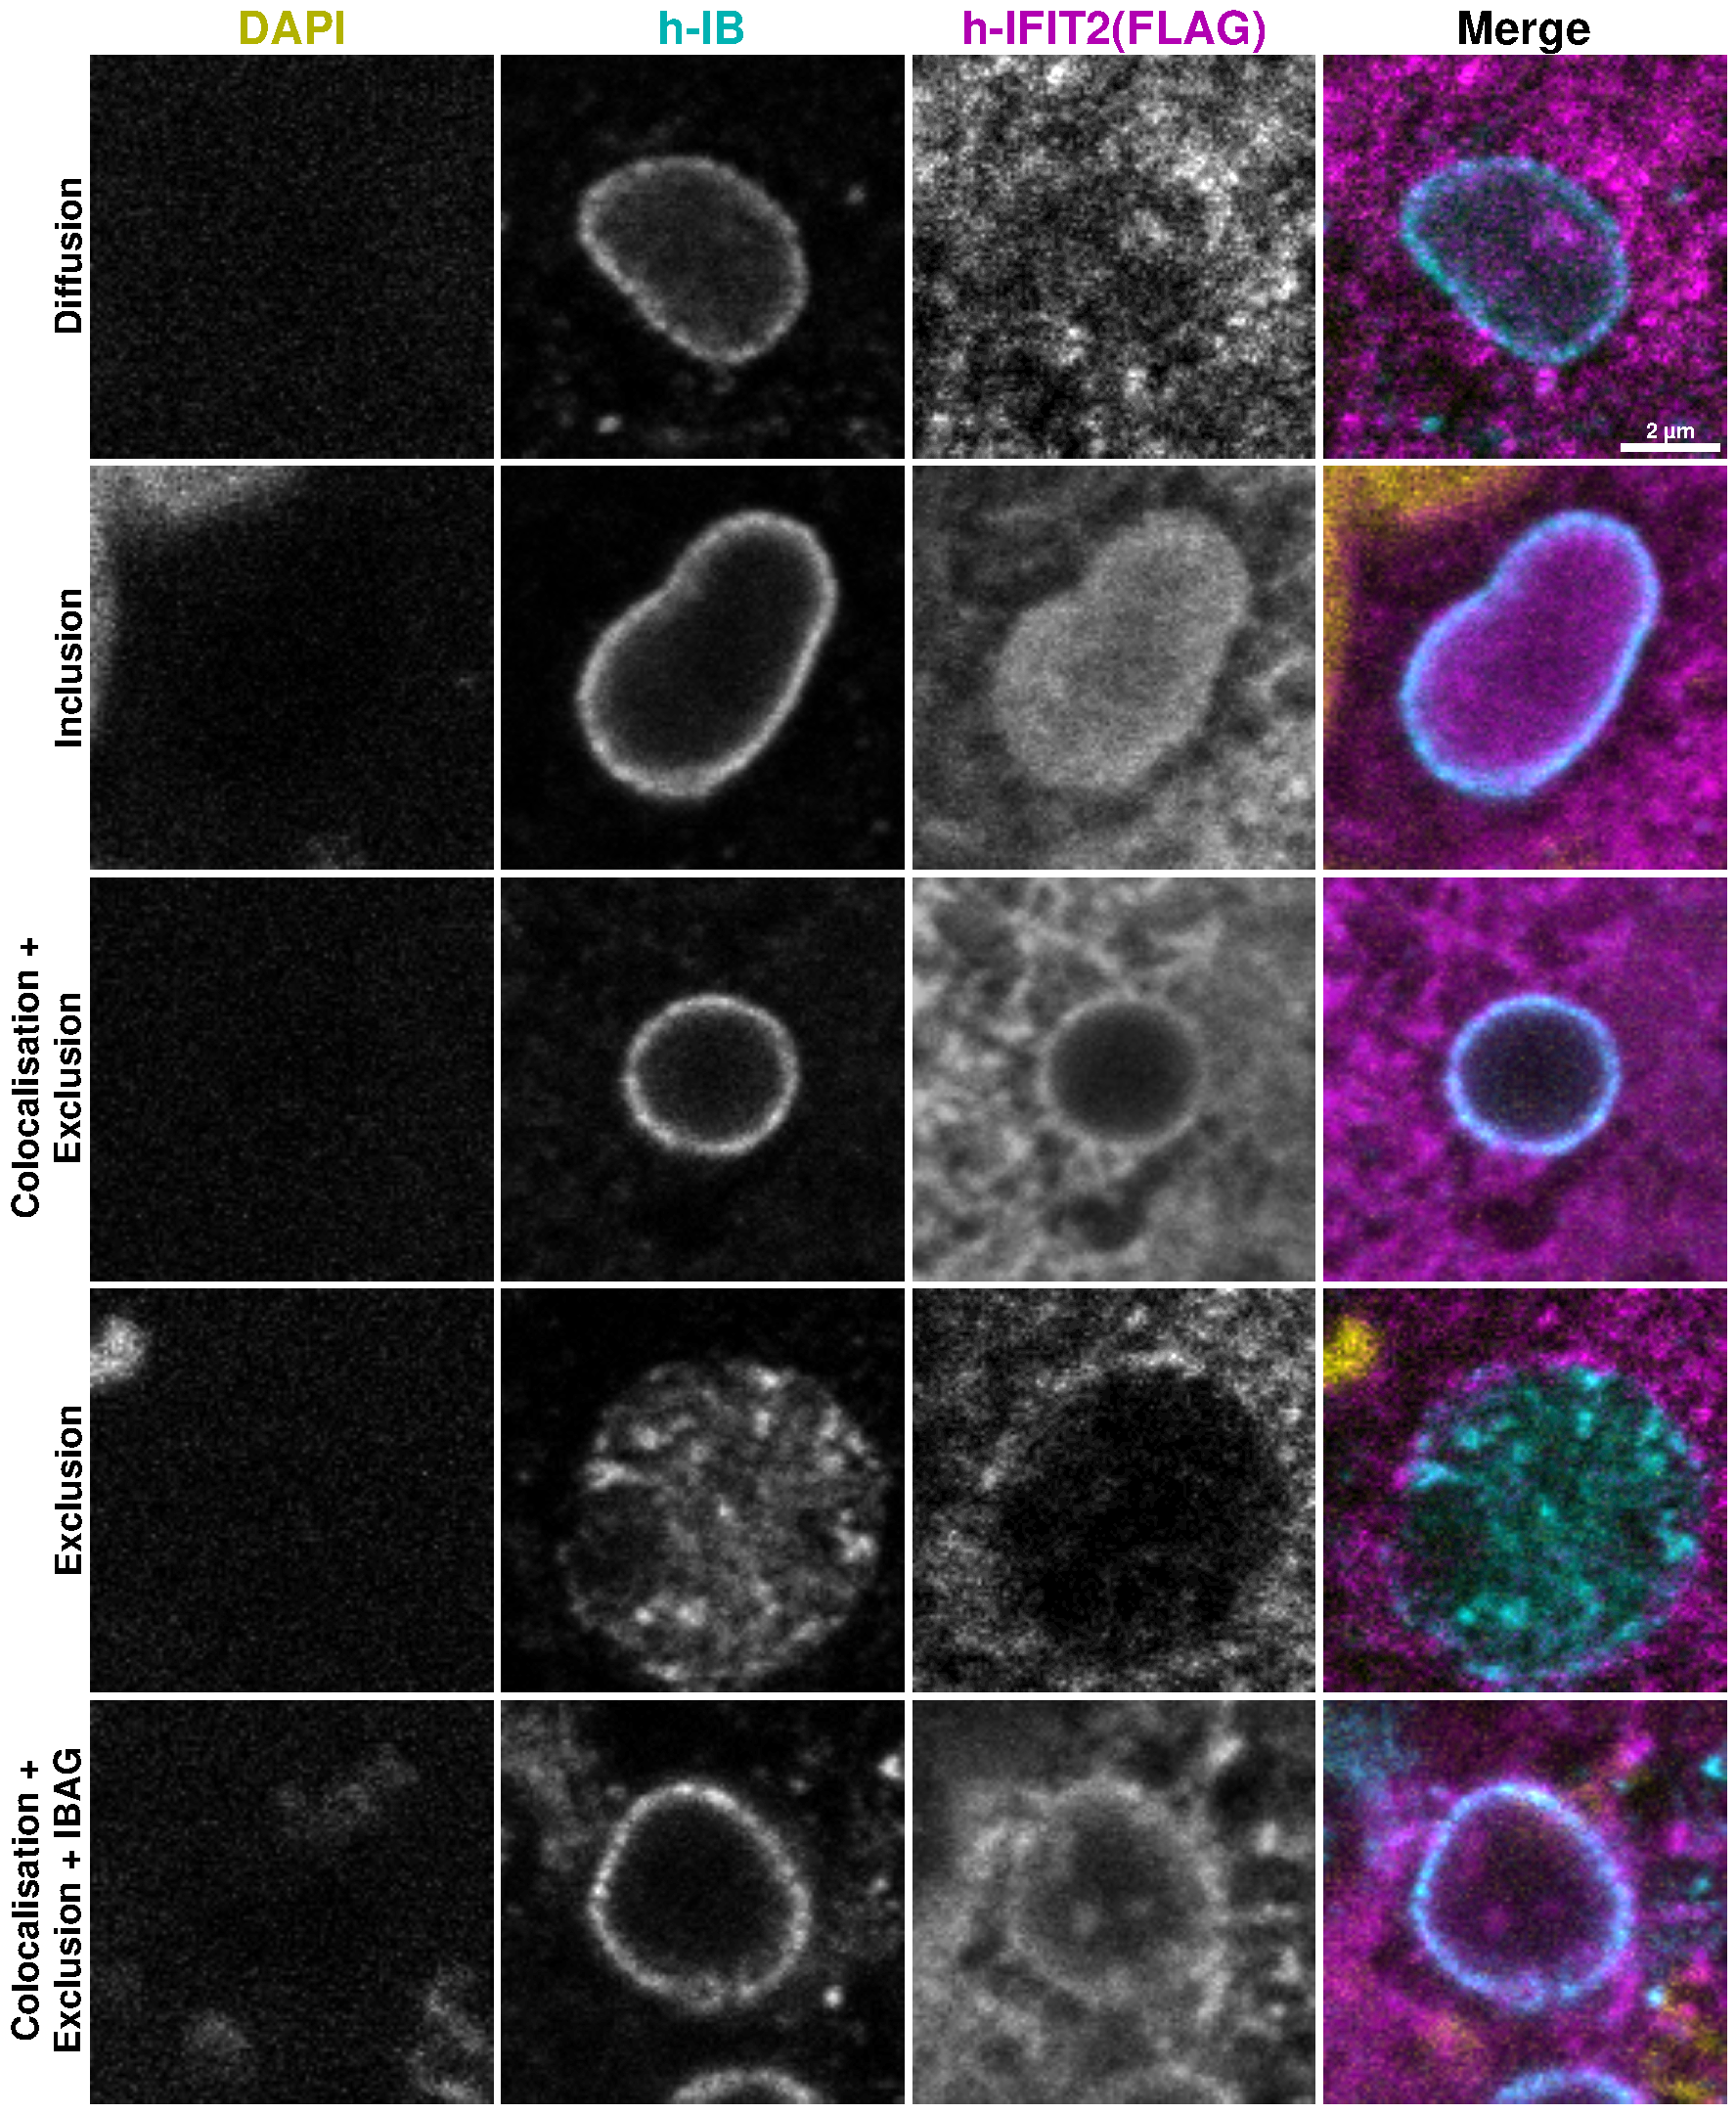
\includegraphics[width=1\linewidth]{09. Chapter 4/Figs/02. Overexpression/02. IFIT2/03. hi2f-hrsv.pdf}
    \caption[Representative Images of Observed Phenotypes of Exogenous hIFIT2 in the Context of hRSV Inclusion Bodies in Vero Cell Line.]{\textbf{Representative Images of Observed Phenotypes of Exogenous hIFIT2 in the Context of hRSV Inclusion Bodies in Vero Cell Line.} Vero cells were infected with human RSV at MOI 1. 24 HPI, the cells were transfected with hIFIT2-FLAG containing plasmids using TransIT-X2 and were fixed after a further 24 hours. Cellular nuclei were stained with DAPI (yellow), and cells were double-labelled with anti-RSV N (cyan) and anti-FLAG (magenta) antibodies. This figure showcases representative examples of relevant phenotypes in the interaction between exogenous hIFIT2 and hRSV inclusion bodies. These phenotypes are presented in descending order based on their percentage proportions. The scale bar indicates 2 \(\mu \mbox{m}\).}
    \label{fig:Representative Images of Observed Phenotypes of Exogenous hIFIT2 in the Context of hRSV Inclusion Bodies in Vero Cell Line}
\end{figure}

48 21 14 9 5
0.9 2.1 7 11 32

In the follow up experiment, exogenous bovine IFIT2 in the context of human RSV infection shows the same two phenotypes. It is either excluded from the IBs (middle panel) or colocalises with the ring structure of the IBs (top and bottom panel; highlighted with arrows).

\begin{figure}
    \begin{subfigure}{0.495\textwidth}
        \caption{}
        \includegraphics[width=1\linewidth]{09. Chapter 4/Figs/02. Overexpression/02. IFIT2/04. bar_bi2f_hrsv.pdf} 
    \end{subfigure}
    \begin{subfigure}{0.495\textwidth}
        \caption{}
        \includegraphics[width=1\linewidth]{09. Chapter 4/Figs/02. Overexpression/02. IFIT2/05. box_bi2f_hrsv.pdf}
    \end{subfigure}
    \caption[Observed Phenotypes of Exogenous bIFIT2 in the Context of hRSV Inclusion Bodies in Vero Cell Line.]{\textbf{Observed Phenotypes of Exogenous bIFIT2 in the Context of hRSV Inclusion Bodies in Vero Cell Line.} Vero cells were infected with human RSV at MOI 1. 24 HPI, the cells were transfected with bIFIT2-FLAG containing plasmids using TransIT-X2 and were fixed after a further 24 hours. Cells were labelled with anti-RSV N and anti-FLAG antibodies and imaged on a confocal microscope. Panel (a) shows the percentual proportions of observed phenotypes between hRSV inclusion bodies and exogenous bIFIT2 (62 observations), with the red dotted line denoting the 5\% threshold, marking phenotypes considered relevant above this limit. Panel (b) shows the IB area in \(\mu \mbox{m}^2\) per observed relevant phenotype.}
    \label{fig:Observed Phenotypes of Exogenous bIFIT2 in the Context of hRSV Inclusion Bodies in Vero Cell Line}
\end{figure}

\begin{figure}
    \centering
    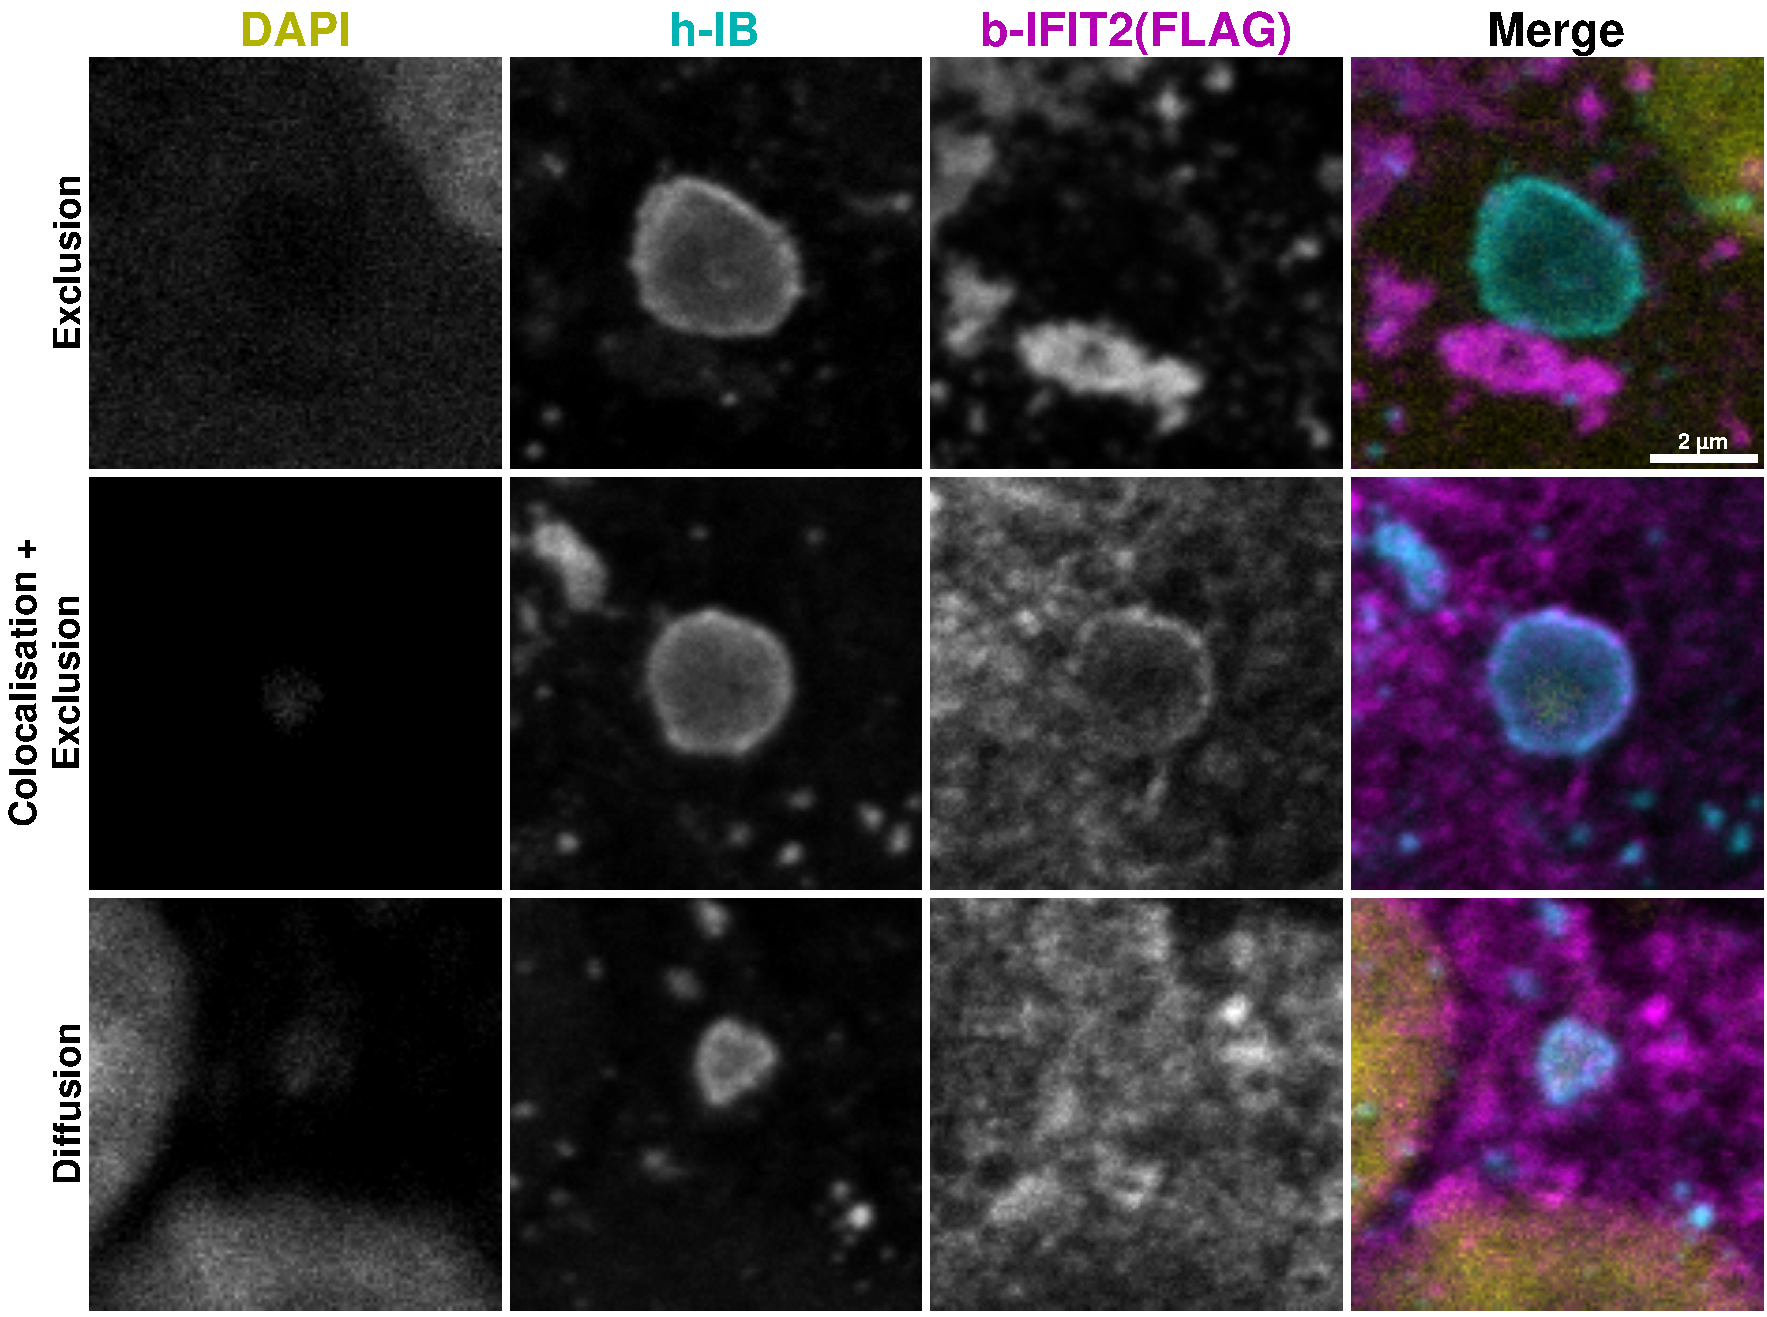
\includegraphics[width=1\linewidth]{09. Chapter 4/Figs/02. Overexpression/02. IFIT2/06. bi2f-hrsv.pdf}
    \caption[Representative Images of Observed Phenotypes of Exogenous bIFIT2 in the Context of hRSV Inclusion Bodies in Vero Cell Line.]{\textbf{Representative Images of Observed Phenotypes of Exogenous bIFIT2 in the Context of hRSV Inclusion Bodies in Vero Cell Line.} Vero cells were infected with human RSV at MOI 1. 24 HPI, the cells were transfected with bIFIT2-FLAG containing plasmids using TransIT-X2 and were fixed after a further 24 hours. Cellular nuclei were stained with DAPI (yellow), and cells were double-labelled with anti-RSV N (cyan) and anti-FLAG (magenta) antibodies. This figure showcases representative examples of relevant phenotypes in the interaction between exogenous bIFIT2 and hRSV inclusion bodies. These phenotypes are presented in descending order based on their percentage proportions. The scale bar indicates 2 \(\mu \mbox{m}\).}
    \label{fig:Representative Images of Observed Phenotypes of Exogenous bIFIT2 in the Context of hRSV Inclusion Bodies in Vero Cell Line}
\end{figure}

66 17 16
1 5 0.5

Exogenous bovine IFIT2 during bovine RSV infection seems to be excluded from the inclusion bodies, although the data is not great and the IFIT2 is aggregated in both cells shown.

\begin{figure}
    \begin{subfigure}{0.495\textwidth}
        \caption{}
        \includegraphics[width=1\linewidth]{09. Chapter 4/Figs/02. Overexpression/02. IFIT2/07. bar_bi2f_brsv.pdf} 
    \end{subfigure}
    \begin{subfigure}{0.495\textwidth}
        \caption{}
        \includegraphics[width=1\linewidth]{09. Chapter 4/Figs/02. Overexpression/02. IFIT2/08. box_bi2f_brsv.pdf}
    \end{subfigure}
    \caption[Observed Phenotypes of Exogenous bIFIT2 in the Context of bRSV Inclusion Bodies in Vero Cell Line.]{\textbf{Observed Phenotypes of Exogenous bIFIT2 in the Context of bRSV Inclusion Bodies in Vero Cell Line.} Vero cells were infected with human RSV at MOI 1. 24 HPI, the cells were transfected with bIFIT2-FLAG containing plasmids using TransIT-X2 and were fixed after a further 24 hours. Cells were labelled with anti-RSV N and anti-FLAG antibodies and imaged on a confocal microscope. Panel (a) shows the percentual proportions of observed phenotypes between bRSV inclusion bodies and exogenous bIFIT2 (31 observations), with the red dotted line denoting the 5\% threshold, marking phenotypes considered relevant above this limit. Panel (b) shows the IB area in \(\mu \mbox{m}^2\) per observed relevant phenotype.}
    \label{fig:Observed Phenotypes of Exogenous bIFIT2 in the Context of bRSV Inclusion Bodies in Vero Cell Line}
\end{figure}

\begin{figure}
    \centering
    \includegraphics[width=1\linewidth]{09. Chapter 4/Figs/02. Overexpression/02. IFIT2/09. bi2f-brsv.pdf}
    \caption[Representative Images of Observed Phenotypes of Exogenous bIFIT2 in the Context of bRSV Inclusion Bodies in Vero Cell Line.]{\textbf{Representative Images of Observed Phenotypes of Exogenous bIFIT2 in the Context of bRSV Inclusion Bodies in Vero Cell Line.} Vero cells were infected with human RSV at MOI 1. 24 HPI, the cells were transfected with bIFIT2-FLAG containing plasmids using TransIT-X2 and were fixed after a further 24 hours. Cellular nuclei were stained with DAPI (yellow), and cells were double-labelled with anti-RSV N (cyan) and anti-FLAG (magenta) antibodies. This figure showcases representative examples of relevant phenotypes in the interaction between exogenous bIFIT2 and bRSV inclusion bodies. These phenotypes are presented in descending order based on their percentage proportions. The scale bar indicates 2 \(\mu \mbox{m}\).}
    \label{fig:Representative Images of Observed Phenotypes of Exogenous bIFIT2 in the Context of bRSV Inclusion Bodies in Vero Cell Line}
\end{figure}

94 6
3.9 1.3

\subsection{Endeavour in Understanding the Mechanisms of IFIT2-RSV IB Interaction} \label{subsec:Endeavour in Understanding the Mechanisms of IFIT2-RSV IB Interaction}
%The Generation of Bovine IFIT2 RNA-Binding Mutant
Using published data about hIFIT2 rna-binding mutant

Difficulty of using alpha-fold with IFIT2 due to the swap domain

Using SWISS-MODEL to predict bIFIT2 structure from published hIFIT2 structures

Alignment of both structures, assessment of electrostatic charges and establishment of residues to be mutated

Primer design and mutagenesis procedure based on published hIFIT2 RNA-binding mutant paper
\cite{Tran2020InfluenzaMRNAs}

\ref{subsec:PCR for Point Mutant Generation}

\begin{figure}
    \centering
    \includegraphics[width=1\linewidth]{09. Chapter 4/Figs/01. pIB/03. IFIT2/05. IFIT2-RNA binding mutant/01. Structure/01. structure.png}
    \caption[ifit2 mutant structure]{\textbf{bifit2 mutant structure.} write caption}
    \label{fig:ifit2 mutant structure}
\end{figure}


\begin{figure}
    \begin{subfigure}{0.495\textwidth}
        \caption{}
        \includegraphics[width=1\linewidth]{09. Chapter 4/Figs/01. pIB/03. IFIT2/05. IFIT2-RNA binding mutant/02. pIB/01. bar_bi2f24_hnhp.pdf} 
    \end{subfigure}
    \begin{subfigure}{0.495\textwidth}
        \caption{}
        \includegraphics[width=1\linewidth]{09. Chapter 4/Figs/01. pIB/03. IFIT2/05. IFIT2-RNA binding mutant/02. pIB/02. box_bi2f24_hnhp.pdf}
    \end{subfigure}
    \caption[Diverse Phenotypic Interactions of Bovine IFIT2 RNA-Binding Mutant with Human RSV Pseudo Inclusion Bodies (pIBs) in the Vero Cell Line.]{\textbf{Diverse Phenotypic Interactions of Bovine IFIT2 RNA-Binding Mutant with Human RSV Pseudo Inclusion Bodies (pIBs) in the Vero Cell Line.} Vero cells were transfected with hRSV N and P, along with bovine IFIT2-FLAG RNA-binding mutant containing plasmids using TransIT-X2 and were fixed after 24 hours. Cells were labelled with anti-RSV N and anti-FLAG antibodies and imaged on a confocal microscope. Panel (a) shows percentual proportions of observed phenotypes between hRSV pseudo inclusion bodies and exogenous bovine IFIT2-FLAG RNA-binding mutant (548 observations), with the red dotted line denoting the 5\% threshold, marking phenotypes considered relevant above this limit. Panel (b) shows the IB area in \(\mu \mbox{m}^2\) per observed relevant phenotype.}
    \label{fig:Diverse Phenotypic Interactions of Bovine IFIT2 RNA-Binding Mutant with Human RSV Pseudo Inclusion Bodies (pIBs) in the Vero Cell Line}
\end{figure}

\begin{figure}
    \centering
    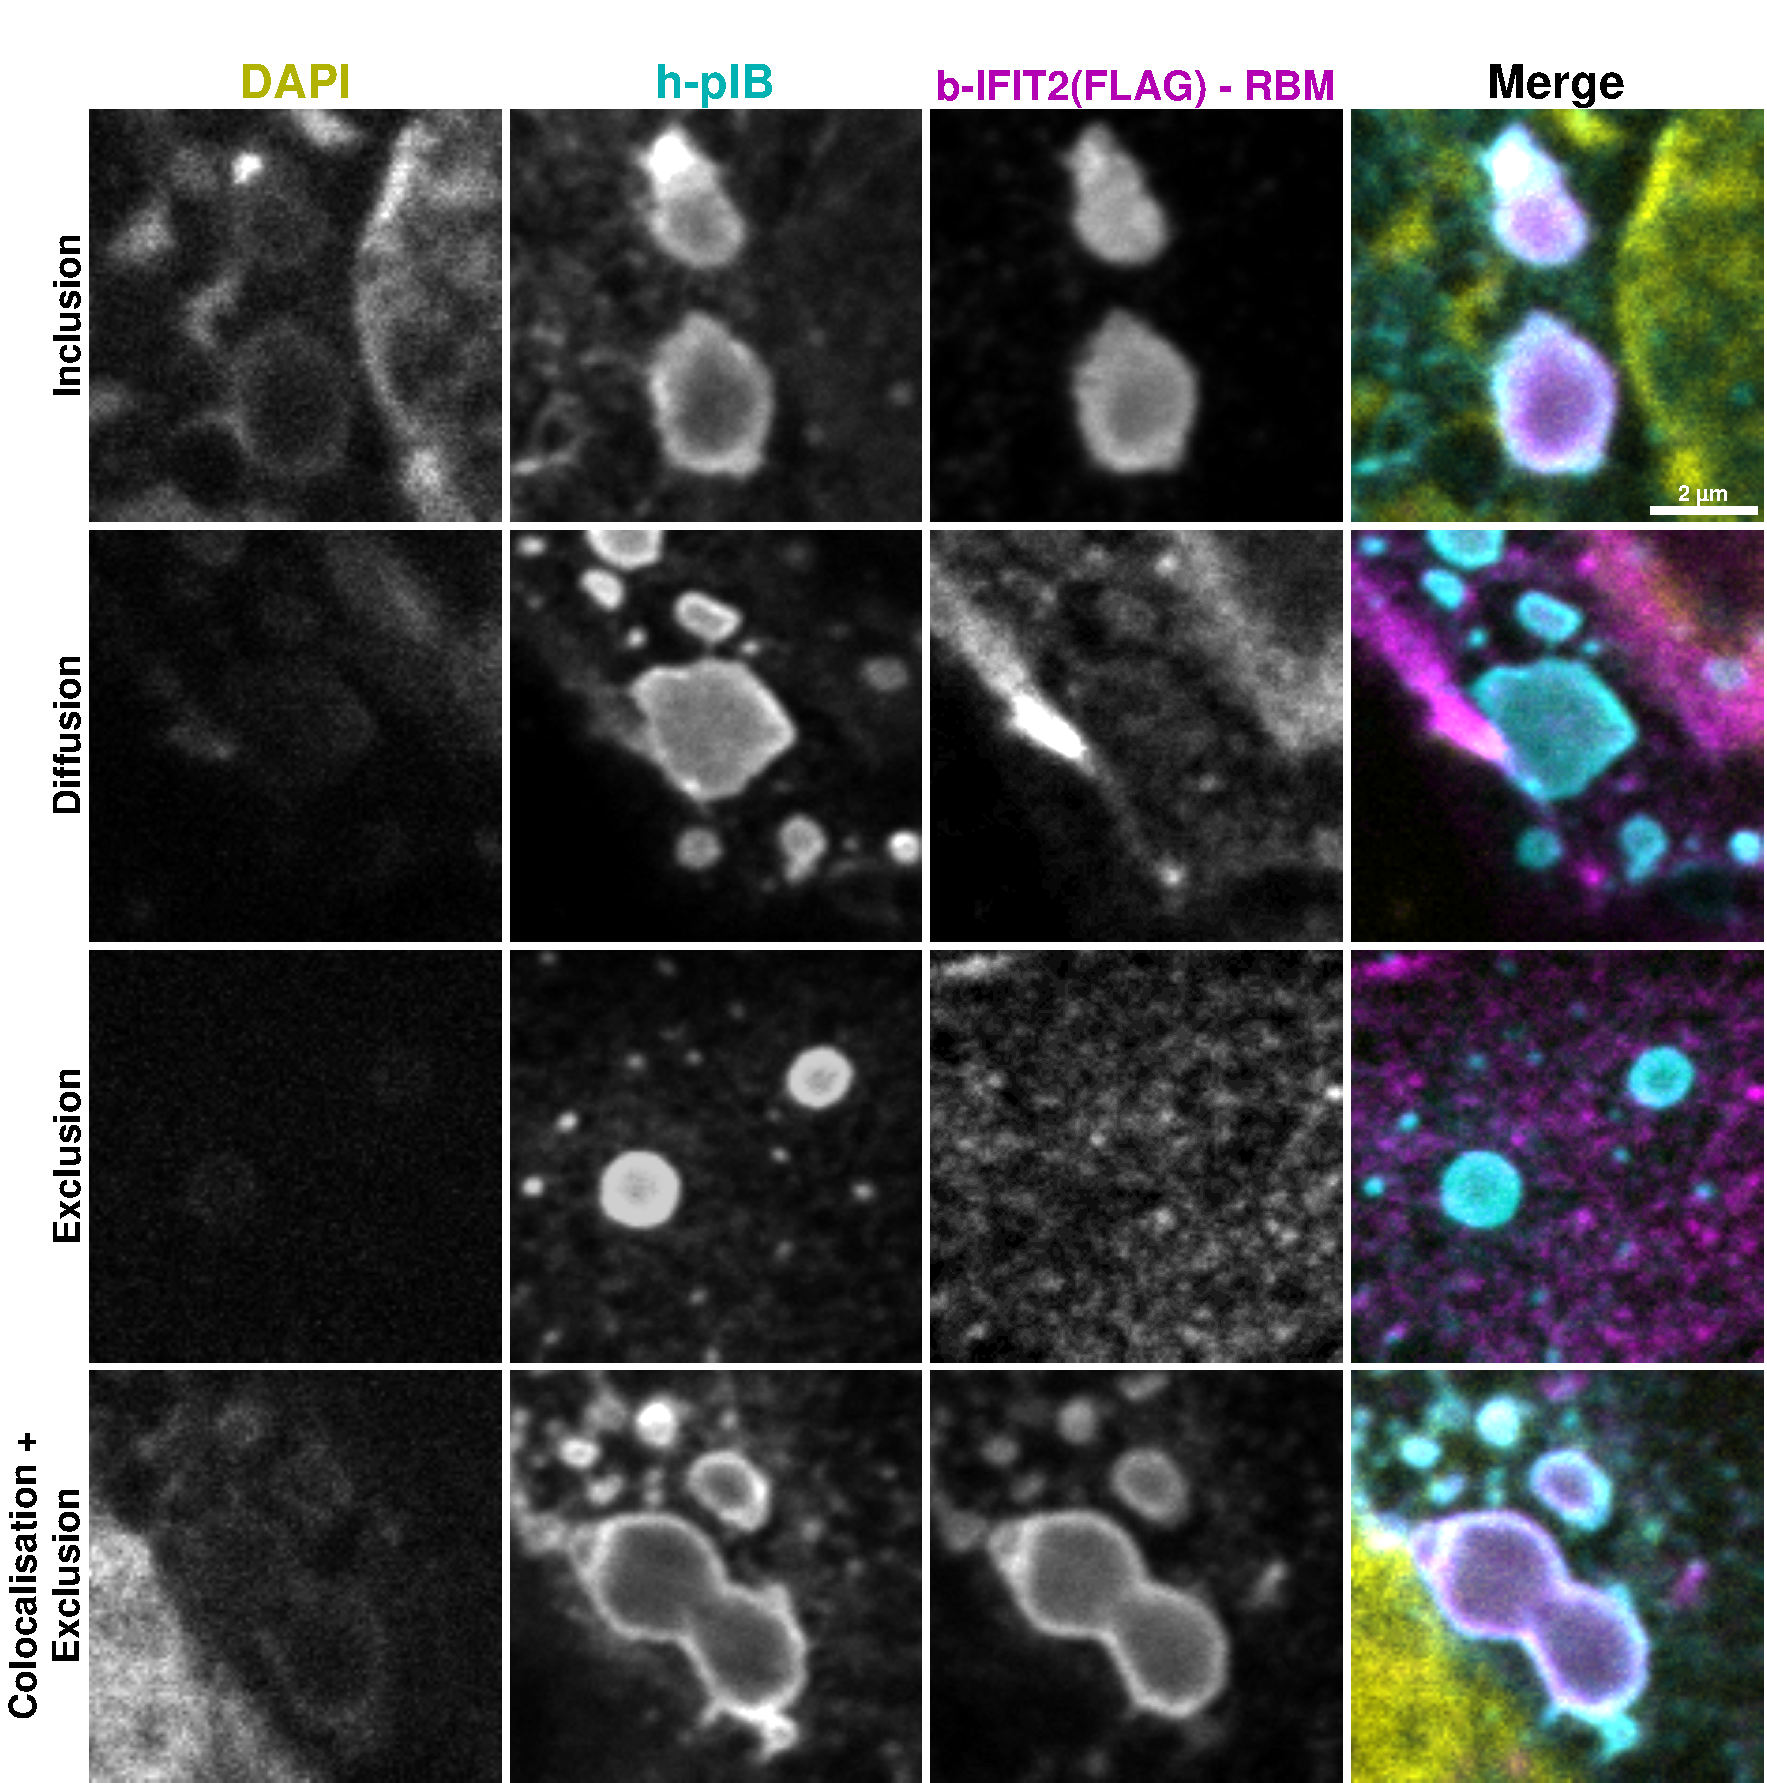
\includegraphics[width=1\linewidth]{09. Chapter 4/Figs/01. pIB/03. IFIT2/05. IFIT2-RNA binding mutant/02. pIB/03. bi2f24-hnhp.pdf}
    \caption[Representative Images of Diverse Phenotypic Interactions of Bovine IFIT2 RNA-Binding Mutant with Human RSV Pseudo Inclusion Bodies (pIBs) in the Vero Cell Line.]{\textbf{Representative Images of Diverse Phenotypic Interactions of Bovine IFIT2 RNA-Binding Mutant with Human RSV Pseudo Inclusion Bodies (pIBs) in the Vero Cell Line.}  Vero cells were transfected with bRSV N and P, along with bovine IFIT2-FLAG RNA-binding mutant containing plasmids using TransIT-X2 and were fixed after 24 hours. Cellular nuclei were stained with DAPI (yellow), and cells were double-labelled with anti-RSV N (cyan) and anti-FLAG (magenta) antibodies. This figure showcases representative examples of relevant phenotypes in the interaction between exogenous bovine IFIT2-FLAG RNA-binding mutant and hRSV pseudo-inclusion bodies. These phenotypes are presented in descending order based on their percentage proportions. The scale bar indicates 2 \(\mu \mbox{m}\).}
    \label{fig:Representative Images of Diverse Phenotypic Interactions of Bovine IFIT2 RNA-Binding Mutant with Human RSV Pseudo Inclusion Bodies (pIBs) in the Vero Cell Line}
\end{figure}

49 27 13 11
0.8 0.5 1 1.8

\begin{figure}
    \begin{subfigure}{0.495\textwidth}
        \caption{}
        \includegraphics[width=1\linewidth]{09. Chapter 4/Figs/01. pIB/03. IFIT2/05. IFIT2-RNA binding mutant/02. pIB/04. bar_bi2f24_bnbp.pdf} 
    \end{subfigure}
    \begin{subfigure}{0.495\textwidth}
        \caption{}
        \includegraphics[width=1\linewidth]{09. Chapter 4/Figs/01. pIB/03. IFIT2/05. IFIT2-RNA binding mutant/02. pIB/05. box_bi2f24_bnbp.pdf}
    \end{subfigure}
    \caption[Diverse Phenotypic Interactions of Bovine IFIT2 RNA-Binding Mutant with Bovine RSV Pseudo Inclusion Bodies (pIBs) in the Vero Cell Line.]{\textbf{Diverse Phenotypic Interactions of Bovine IFIT2 RNA-Binding Mutant with Bovine RSV Pseudo Inclusion Bodies (pIBs) in the Vero Cell Line.} Vero cells were transfected with bRSV N and P, along with bovine IFIT2-FLAG RNA-binding mutant containing plasmids using TransIT-X2 and were fixed after 24 hours. Cells were labelled with anti-RSV N and anti-FLAG antibodies and imaged on a confocal microscope. Panel (a) shows percentual proportions of observed phenotypes between bRSV pseudo inclusion bodies and exogenous bovine IFIT2-FLAG RNA-binding mutant (2 observations), with the red dotted line denoting the 5\% threshold, marking phenotypes considered relevant above this limit. Panel (b) shows the IB area in \(\mu \mbox{m}^2\) per observed relevant phenotype.}
    \label{fig:Diverse Phenotypic Interactions of Bovine IFIT2 RNA-Binding Mutant with Bovine RSV Pseudo Inclusion Bodies (pIBs) in the Vero Cell Line}
\end{figure}

\begin{figure}
    \centering
    \includegraphics[width=1\linewidth]{09. Chapter 4/Figs/01. pIB/03. IFIT2/05. IFIT2-RNA binding mutant/02. pIB/06. bi2f24-bnbp.pdf}
    \caption[Representative Images of Diverse Phenotypic Interactions of Bovine IFIT2 RNA-Binding Mutant with Bovine RSV Pseudo Inclusion Bodies (pIBs) in the Vero Cell Line.]{\textbf{Representative Images of Diverse Phenotypic Interactions of Bovine IFIT2 RNA-Binding Mutant with Bovine RSV Pseudo Inclusion Bodies (pIBs) in the Vero Cell Line.}  Vero cells were transfected with bRSV N and P, along with bovine IFIT2-FLAG RNA-binding mutant containing plasmids using TransIT-X2 and were fixed after 24 hours. Cellular nuclei were stained with DAPI (yellow), and cells were double-labelled with anti-RSV N (cyan) and anti-FLAG (magenta) antibodies. This figure showcases representative examples of relevant phenotypes in the interaction between exogenous bovine IFIT2-FLAG RNA-binding mutant and bRSV pseudo inclusion bodies. These phenotypes are presented in descending order based on their percentage proportions. The scale bar indicates 2 \(\mu \mbox{m}\).}
    \label{fig:Representative Images of Diverse Phenotypic Interactions of Bovine IFIT2 RNA-Binding Mutant with Bovine RSV Pseudo Inclusion Bodies (pIBs) in the Vero Cell Line}
\end{figure}

100
1.8

% summary i2
We have described how bovine IFIT2 RNA-binding mutant was designed based on the published human IFIT2 RNA-binding mutant data (needs to be annotated more). Overexpression of bovine IFIT2 RNA-binding mutant yields cellular distribution and morphology similar to what was observed with overexpressing human IFIT2-FLAG, suggesting that the mutant proteins are not toxic to the cells. In the first experiment where we were looking at interaction between bovine IFIT2 RNA-binding mutant and human pseudo inclusion bodies we saw several phenotypes. We observed bovine IFIT2 RNA-binding mutant being excluded from small and big pIBs and pIB associated filamentous network, while fully or partially colocalising with other pIBs. In a subsequent experiment we observed only colocalization and inclusion formation. When assessing the interaction between bovine IFIT2 RNA-binding mutant and human pIBs formed using wild-type human RSV P and GFP-tagged human RSV N, we observed consistently in two experiments that bovine IFIT2 RNA-binding mutant colocalises to the pIB structures.